% update the discussion of Level 2 future
% mention 'reversible' flag is necessary b/c kineticLaw is optional
% need update schema to use ``annotation''

\documentclass[10pt]{cekarticle}
\usepackage{amsmath}
\usepackage{amssymb}
\usepackage{array}
\usepackage{wrapfig}
\latexhtml{
%begin{latexonly}
  \usepackage[american]{varioref}
%end{latexonly}
}{
  \newcommand{\vref}[1]{\ref{#1}}
}

% I should use cekarticle2, but it's not finished and I don't have time to
% fix the problems now.  So, I'm importing the color code.

% Test whether we're being run from latex or latex2html
\latexhtml{
  % For latex.
  % Test whether we're being run from pdflatex or regular latex.
  \ifx\pdfoutput\undefined
    % Regular latex.
    \if@xdvi
      \RequirePackage[xdvi,usenames]{color}
    \else
      \RequirePackage[dvips,usenames]{color}
    \fi
  \else
    % Pdflatex.
    \RequirePackage[pdftex,usenames]{color}
    \definecolor{MidnightBlue}{cmyk}{0.98,0.13,0,0.43}
    \definecolor{OliveGreen}{cmyk}{0.64,0,0.95,0.40}
    \definecolor{BrickRed}{cmyk}{0,0.89,0.94,0.28}
    \definecolor{RawSienna}{cmyk}{0,0.72,1,0.45}
  \fi
}{
  % For latex2html.
  \RequirePackage[usenames]{color}
}

\RequirePackage{colortbl}

% Miscellaneous macros.

\newcommand{\D}{\displaystyle}
\newcommand{\tm}{\textsuperscript{\tiny{\texttrademark}}}
\newcommand{\changed}[1]{\textcolor{BrickRed}{#1}}
\newenvironment{blockChanged}{\color{BrickRed}}{\color{black}}

\begin{document}

%=============================================================================
% Title page
%=============================================================================

\title{\mbox{Systems Biology Markup Language (SBML) Level 1:}\\
  Structures and Facilities for Basic Model Definitions}

\author{Michael Hucka, Andrew Finney, Herbert Sauro, Hamid Bolouri}

\authoremail{\{mhucka,afinney,hsauro,hbolouri\}@cds.caltech.edu}

\address{Systems Biology Workbench Development Group\\
  JST ERATO Kitano Symbiotic Systems Project\\
  Control and Dynamical Systems, MC 107-81\\
  California Institute of Technology, Pasadena, CA 91125, USA\\[3pt]
  \url{http://www.cds.caltech.edu/erato}}

\acknowledge{Principal Investigators: John Doyle and Hiroaki Kitano}

% The last vspace with the negative arg is a wreched hack to get the toc
% to fit on the first page even though I've put a date on a separate line
% and thus increased the vertical needs over what they were in the L1v1 doc.

\date{\vspace*{-1ex}SBML Level 1, \changed{Version 2 (Final)}\\[3pt]
  \changed{28 August 2003}\vspace*{-10pt}}

\renewcommand{\baselinestretch}{0.96}
\maketitlepage
\renewcommand{\baselinestretch}{0.98}


%=============================================================================
\section{Introduction}
\label{sec:introduction}
%=============================================================================

We present the \textbf{S}ystems \textbf{B}iology \textbf{M}arkup
\textbf{L}anguage (SBML) Level~1\changed{, Version 2}, a description
language for simulations in systems biology.  SBML is oriented towards
representing biochemical networks common in research on a number of topics,
including cell signaling pathways, metabolic pathways, biochemical
reactions, gene regulation, and many others.  A recent
conference~\citep{kitano:2001} highlights the range of topics that fall
under the umbrella of \emph{systems biology} and are in the domain of the
description language defined here.  Many contemporary research initiatives
demonstrate the growing popularity of this kind of multidisciplinary
work~\cite[e.g.,][]{abbott:1999,gilman:2000,popel:1998,smaglik:2000,smaglik:2000b}.

SBML Level~1 is the result of merging modeling-language features from the
following simulation systems: \emph{BioSpice}~\citep{arkin:2001},
\emph{DBSolve}~\citep{goryanin:2001,goryanin:1999},
\emph{E-Cell}~\citep{tomita:1999,tomita:2001},
\emph{Gepasi}~\citep{mendes:1997,mendes:2001},
\emph{Jarnac}~\citep{sauro:2000,sauro:1991},
\emph{StochSim}~\citep{bray:2001,morton-firth:1998}, and \emph{Virtual
  Cell}~\citep{schaff:2000,schaff:2001}.  SBML was developed with the help
of the authors of these packages.  As a result of being based on actual
working simulation software, it is a practical and functional description
language.  Our goal in creating it has been to provide an open standard
that will enable simulation software to exchange models, something that is
currently impossible because there is no standard model exchange language.
We expect SBML models to be encoded using XML, the eXtensible Markup
Language~\citep{bosak:1999,bray:1998}, and we include here an XML Schema
that defines SBML Level~1.

%-----------------------------------------------------------------------------
\subsection{\changed{Summary of Changes in Version 2 of SBML Level 1}}
%-----------------------------------------------------------------------------

\begin{blockChanged}
  This document describes Version 2 of SBML Level 1.  Changes with respect
  to Version~1 of the SBML specification are indicated in red.  Most
  changes in this document are simply textual changes made in an attempt to
  clarify the language of the specification and to correct typographical
  and other small errors.  The following list is an overview of the more
  notable changes:
\vspace*{-1ex}\begin{itemize}\setlength{\parskip}{0.27ex}
  
\item SBML Level 1 Version 2 deprecates the spelling \emph{specie} 
  in favor of \emph{species}.
  
\item There are additional names in the list of reserved XML Namespaces in
  Table~\ref{tab:reserved-urls}. (Section~\ref{sec:annotation-guidelines}.)

\item The specified syntax of \class{SName} now corresponds to the intended
  syntax (Section~\ref{sec:name}), and the syntax is expressed using the
  variant of EBNF used by the XML 1.0 specification.

\item Table~\vref{tab:reserved-names} no longer lists ``\texttt{umar}'' twice.

\item The default scale of units is now correctly defined as zero.
  (Section~\ref{sec:unitdefinitions}.)
  
\item Compartments are now optional (Section~\ref{sec:compartments});
  however, each species in a model is still required to be located in a
  compartment, which means that for all meaningful models, compartments are
  mandatory.

\item Species are now optional.  (Section~\ref{sec:species}.)

\item The \attrib{value} of a parameter is now optional.
  (Section~\ref{sec:parameters}.)
  
\item The section on rules has greater detail on the intended use and
  limitations of rules.  (Section~\ref{sec:rules}.)
  
\item Reactions are optional, and lists of reactants and products in a
  reaction may be empty.  (Section~\ref{sec:reactions}.)
  
\item The values of attributes on \class{speciesReference} are required to
  be positive numbers; also, Section~\ref{subsec:speciesreference} is now
  more explicit about the intended use of \class{speciesReference}.
  
\item The example given in Section~\ref{subsection:ruleseg} is a different,
  corrected example.
  
\item The rate laws in Appendix~\ref{apdx:predefined-functions} are more
  correct and consistent.  In addition, the law \texttt{massr} is no longer
  defined because its definition posed parsing problems and it was
  redundant.  The law \texttt{massi} is now called \texttt{mass}.  SBML
  Level~1 Version~1's \texttt{massr} is equivalent to
  ``$\text{mass}[S_i,k_1] - \text{mass}[P_j,k_2]$''.

\item The \attrib{version} attribute of the \class{sbml} element now has a
  value of ``\texttt{2}'' instead of ``\texttt{1}''.
  
\end{itemize}

In addition, we have established the web site \url{http://www.sbml.org} as
the home site for SBML, and all documents, schemas and software are
available from there.

\end{blockChanged}


%-----------------------------------------------------------------------------
\subsection{Scope and Limitations}
%-----------------------------------------------------------------------------

SBML Level 1 is meant to support non-spatial biochemical models and the
kinds of operations that are possible in existing analysis/simulation
tools.  A number of potentially desirable features have been intentionally
omitted from the language definition.  Future software tools will
undoubtedly require the evolution of SBML; we expect that subsequent
releases of SBML (termed \emph{levels}) will add additional structures and
facilities currently missing from Level~1, once the simulation community
gains experience with the current language definition.  In
Section~\ref{sec:level-2}, we discuss extensions that will likely be
included in SBML Level~2 \changed{or 3}.

The definition of the model description language presented here does not
specify \emph{how} programs should communicate or read/write SBML.  We
assume that for a simulation program to communicate a model encoded in
SBML, the program will have to translate its internal data structures to
and from SBML, use a suitable transmission medium and protocol, etc., but
these issues are outside of the scope of this document.


%-----------------------------------------------------------------------------
\subsection{Notational Conventions}
%-----------------------------------------------------------------------------

SBML is intended to be a common XML-based format for encoding systems
biology models in a simple form that software tools can use as an exchange
format.  However, for easier communication to human readers, we define SBML
using a graphical notation based upon UML, the Unified Modeling
Language~\citep{eriksson:1998,oestereich:1999}.  This UML-based definition
in turn is used to define an XML
Schema~\citep{biron:2000,fallside:2000,thompson:2000} for SBML.  There are
three main advantages to using UML as a basis for defining SBML data
structures.  First, compared to using other notations or a programming
language, the UML visual representations are generally easier to grasp by
readers who are not computer scientists.  Second, the visual notation is
implementation-neutral: the defined structures can be encoded in any
concrete implementation language---not just XML, but C or Java as well.
Third, UML is a de facto industry standard that is documented in many
sources.  Readers are therefore more likely to be familiar with it than
other notations.

Our notation and our approach for mapping UML to XML Schemas is explained
in a separate document~\citep{hucka:2000b}.  A summary of the essential
points is presented in Appendix~\ref{apdx:notation}, and examples
throughout this document illustrate the approach.  We also follow certain
naming and typographical conventions throughout this document.
Specifically, the names of data structure attributes or fields begin with a
lowercase letter, and the names of data structures and types begin with an
uppercase letter.  Keywords (names of types, XML elements, etc.) are
written in a typewriter-style font; for example, \class{Compartment} is a
type name and \class{compartment} is a field name.  Likewise, literal XML
examples are also written in a typewriter-style font.


%=============================================================================
\section{Overview of SBML}
\label{sec:overview}
%=============================================================================

\begin{wrapfigure}[5]{r}{2.5 in}
\begin{center}
\vspace*{-2ex}
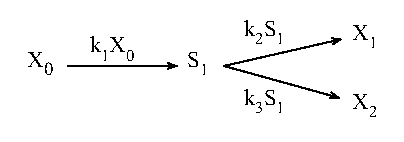
\includegraphics[scale = 0.85]{figs/example-network}
\end{center}
\end{wrapfigure}
\changed{The example on the right is a simple, hypothetical network of
  biochemical reactions that can be represented in SBML.}  Broken down into
its constituents, this model contains a number of components: reactant
species, product species, reactions, rate laws, and parameters in the rate
laws.

To analyze or simulate this network, additional components must be made
explicit, including compartments for the species, and units on the various
quantities.  The top level of an SBML model definition simply consists of
lists of these components:
\begin{center}
  \slshape
  \begin{tabular}{c}
    \begin{minipage}{3in}
      \begin{tabbing}
        xxxx\=xxxx\=xxxx\=xxxx\=\kill
        beginning of model definition\\
        \>list of unit definitions\\
        \>list of compartments\\
        \>list of species\\
        \>list of parameters\\
        \>list of rules\\
        \>list of reactions\\
        end of model definition
      \end{tabbing}
    \end{minipage}
  \end{tabular}
\end{center}
The meaning of each component is as follows:
\begin{description}
  
\item \emph{Unit definition}: A name for a unit used in the expression of
  quantities in a model.  Units may be supplied in a number of contexts in
  an SBML model, and it is convenient to have a facility for both setting
  default units and for allowing combinations of units to be given
  abbreviated names.

\item \emph{Compartment}: A container of finite volume for substances.  In
  SBML Level~1, a compartment is primarily a topological structure with a
  volume but no geometric qualities.
  
\item \emph{\changed{Species}}: A substance or entity that takes part in a reaction.
  Some example species are ions such as \changed{$\text{Ca}^{2+}$} and
  molecules such as glucose or ATP.  The primary qualities associated with
  a \changed{species} in SBML Level~1 are its initial amount and the compartment in
  which it is located.
  
\item \emph{Reaction}: A statement describing some transformation,
  transport or binding process that can change the amount of one or more
  species.  For example, a reaction may describe how certain entities
  (reactants) are transformed into certain other entities (products).
  Reactions have associated rate laws describing how quickly they take
  place.
  
\item \emph{Parameter}: A quantity that has a symbolic name.  SBML Level~1
  provides the ability to define parameters that are global to a model as
  well as parameters that are local to a single reaction.
  
\item \emph{Rule}: In SBML, a mathematical expression that is added
  to the differential equations constructed from the set of reactions and
  can be used to set parameter values, establish constraints between
  quantities, etc.

\end{description}

\begin{blockChanged}
A software package can read in a model expressed in SBML and translate it
into its own internal format for model analysis.  For instance, a package
might provide the ability to simulate a model by constructing a set of
differential equations representing the network and then performing
numerical integration on the equations to explore the model's dynamic
behavior.
\end{blockChanged}

SBML allows models of arbitrary complexity to be represented.  Each type of
component in a model is described using a specific type of data structure
that organizes the relevant information.  The data structures determine how
the resulting model is encoded in XML.

In the sections that follow, the various constructs in SBML and their uses
are described in detail.  Section~\ref{sec:general} first introduces a few
basic structures that are used throughout SBML, then
Section~\ref{sec:elements} provides details on each of the main components
of SBML.  Section~\ref{sec:xml-rep} provides several complete examples of
models encoded in XML using SBML.


%=============================================================================
\section{Preliminary Definitions}
\label{sec:general}
%=============================================================================

This section covers certain constructs that are used repeatedly in the rest
of SBML and are useful to discuss before diving into the details of the
components provided in SBML.

%-----------------------------------------------------------------------------
\subsection{Type \class{SBase}}
\label{sec:sbase}
%-----------------------------------------------------------------------------

Each of the main components composing an SBML model definition has a
specific data type that is derived directly or indirectly from a single
\changed{abstract} type called \class{SBase}.  This inheritance hierarchy
is depicted in Figure~\vref{fig:top-level}.

\begin{figure}[ht]
  \centering
  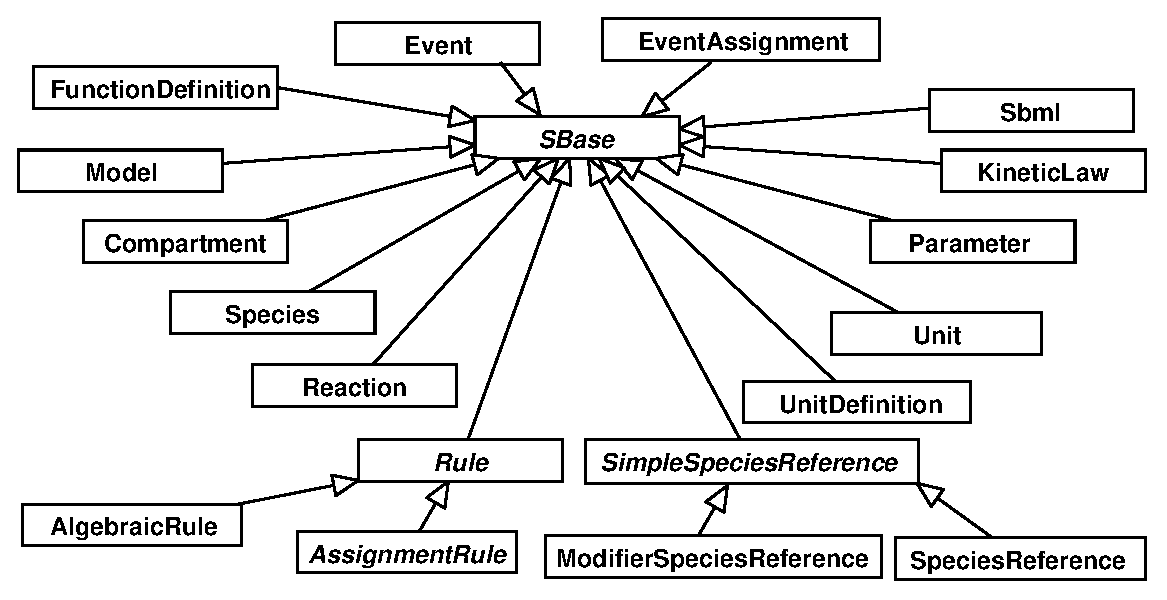
\includegraphics[scale = 0.7]{figs/top-level}
  \caption{A UML diagram of the inheritance hierarchy of major data types
    in SBML.  Open arrows indicate inheritance, pointing from inheritors to 
    their parents~\citep{eriksson:1998,oestereich:1999}.}
  \label{fig:top-level}
\end{figure}

The type \class{SBase} is designed to allow a modeler or a software package
to attach information to each component in an SBML model.  The definition
of \class{SBase} is presented in Figure~\vref{fig:identified}.
\class{SBase} contains two fields, both of which are optional:
\attrib{notes} and \changed{\attrib{annotation}}.  The field \attrib{notes}
is a container for XHTML content.  It is intended for recording optional
user-visible annotations.  Every data object derived directly or indirectly
from type \class{SBase} can have a separate value for \attrib{notes},
allowing users considerable freedom for annotating their models.  The
second field, \changed{\attrib{annotation}}, is provided for
software-generated annotations.  It is a container for arbitrary data (XML
type \class{any}) and is intended to store information not intended for
human viewing.  As with the user-visible \attrib{notes} field, every data
object can have its own \changed{\attrib{annotation}} value.

\begin{figure}[thb]
  \centering
  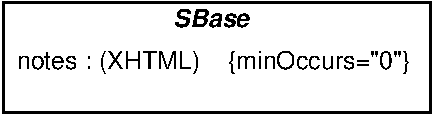
\includegraphics[scale = 0.65]{figs/identified}
  \caption{The definition of \class{SBase}.  Text enclosed in braces next
    to attribute types (i.e., \attribtype{\{minOccurs="1"\}}) indicates
    constraints on the possible attribute values; we use XML Schema
    language to express constraints since we are primarily interested in
    the XML encoding of SBML.}
  \label{fig:identified}
\end{figure}

\changed{The Version~1 specification of SBML Level 1 was inconsistent about
  the spelling of the annotation field.  It named the field
  \attrib{annotation} in Figure~\ref{fig:identified}, but used
  \attrib{annotations} (i.e., plural) in the discussions throughout the
  document.  SBML Level~1 Version~2 clarifies that \attrib{annotation} (singular) is the
  intended name.}

In other type definitions presented below, we follow the UML convention of
eliding the attributes derived from a parent type such as \class{SBase}.
It should be kept in mind that these attributes are always available.



%-----------------------------------------------------------------------------
\subsection{Guidelines for the Use of the \changed{\attrib{annotation}} Field in
  \class{SBase}} 
\label{sec:annotation-guidelines}
%-----------------------------------------------------------------------------

The \changed{\attrib{annotation}} field in the definition of \class{SBase}
is formally unconstrained in order that software developers may attach any
information they need to different components in an SBML model.  However,
it is important that this facility not be misused accidentally.  In
particular, it is critical that information essential to a model definition
is \emph{not} stored in \changed{\attrib{annotation}}.  Parameter values,
functional dependencies between model components, etc., should not be
recorded as annotations.

Here are examples of the kinds of data that may be appropriately stored in
\changed{\attrib{annotation}}: (a) Information about graphical layout of
model components; (b) application-specific processing instructions that do
not change the essence of a model; (c) bibliographic information pertaining
to a given model; and (d) identification information for cross-referencing
components in a model with items in a database.  (We expect to introduce an
explicit scheme for recording bibliographic information and making database
references in \changed{a higher level of SBML}, at which time using
annotations for these purposes will become unnecessary.)

Different applications may use XML Namespaces~\citep{bray:1999} to specify
the intended vocabulary of a particular annotation.  Here is an example of
this kind of usage.  Suppose that a particular application wants to
annotate data structures in an SBML model definition with screen layout
information and a time stamp.  The application developers should choose a
URI (\emph{Universal Resource Identifier}; \citealt{harold:2001,w3c:2000})
reference that uniquely identifies the vocabulary that the
application will use for such annotations, and a prefix string to be used
in the annotations.  For illustration purposes, let us say the URI
reference is ``\texttt{http://www.mysim.org/ns}'' and the prefix is
\texttt{mysim}.  An example of an annotation might then be as follows:

\begin{blockChanged}
\begin{example}
...
<annotation xmlns:mysim="http://www.mysim.org/ns">
    <mysim:nodecolors mysim:bgcolor="green" mysim:fgcolor="white"/>
    <mysim:timestamp>2000-12-18 18:31 PST</mysim:timestamp>
</annotation>
...
\end{example}
\end{blockChanged}

The namespace prefix \texttt{mysim} is used to qualify the XML elements
\texttt{mysim:nodecolors} and \texttt{mysim:timestamp}; presumably these
symbols have meaning to the application.  This example places the XML
Namespace information on \changed{\attrib{annotation}} itself rather than
on a higher-level enclosing construct or the enclosing document level, but
other placements would be valid as well~\citep{bray:1999}.

The use of XML Namespaces permits multiple applications to place
annotations on XML elements of a model without risking interference or
element name collisions.  Annotations stored by different simulation
packages can therefore coexist in the same model definition.  Although XML
Namespace names (``\texttt{http://www.mysim.org/}'' in the example above)
must be URIs references, an XML Namespace name is \emph{not required} to be
directly usable in the sense of identifying an actual, retrieval document
or resource on the Internet~\citep{bray:1999}.  The name is simply intended
to enable unique identification of constructs, and using URIs is a common
and simple way of creating a unique name string.  For the convenience of
\changed{developers of simulation and analysis tools}, we reserve certain
namespace names for use with annotations in SBML.  These reserved names are
listed in Table~\vref{tab:reserved-urls}.

\begin{table}[hb]
  \vspace*{5pt}
  \centering
  \begin{tabular}{ll}
    \toprule
    \changed{\texttt{http://www.sbml.org/2001/ns/basis}}	& \texttt{http://www.sbml.org/2001/ns/jdesigner}\\
    \changed{\texttt{http://www.sbml.org/2001/ns/biocharon}}	& \changed{\texttt{http://www.sbml.org/2001/ns/jigcell}}\\
    \changed{\texttt{http://www.sbml.org/2001/ns/bioreactor}}	& \changed{\texttt{http://www.sbml.org/2001/ns/jsim}}\\
    \changed{\texttt{http://www.sbml.org/2001/ns/biosketchpad}}	& \changed{\texttt{http://www.sbml.org/2001/ns/libsbml}}\\
    \texttt{http://www.sbml.org/2001/ns/biospice}		& \changed{\texttt{http://www.sbml.org/2001/ns/mathsbml}}\\
    \changed{\texttt{http://www.sbml.org/2001/ns/cellerator}}	& \changed{\texttt{http://www.sbml.org/2001/ns/mcell}}\\
    \changed{\texttt{http://www.sbml.org/2001/ns/copasi}}	& \changed{\texttt{http://www.sbml.org/2001/ns/netbuilder}}\\
    \changed{\texttt{http://www.sbml.org/2001/ns/cytoscape}}	& \changed{\texttt{http://www.sbml.org/2001/ns/pathdb}}\\
    \texttt{http://www.sbml.org/2001/ns/dbsolve}		& \changed{\texttt{http://www.sbml.org/2001/ns/promot}}\\
    \texttt{http://www.sbml.org/2001/ns/ecell}			& \changed{\texttt{http://www.sbml.org/2001/ns/sbedit}}\\
    \texttt{http://www.sbml.org/2001/ns/gepasi}			& \changed{\texttt{http://www.sbml.org/2001/ns/sigpath}}\\
    \changed{\texttt{http://www.sbml.org/2001/ns/isys}}		& \texttt{http://www.sbml.org/2001/ns/stochsim}\\
    \texttt{http://www.sbml.org/2001/ns/jarnac}			& \texttt{http://www.sbml.org/2001/ns/vcell}\\
    \bottomrule
  \end{tabular}
  \caption{Reserved XML Namespace names in SBML Level 1 \changed{Version 2}.}
  \label{tab:reserved-urls}
\end{table}

Note that the namespaces being referred to here are XML Namespaces
specifically in the context of the \changed{\attrib{annotation}} field on
\class{SBase}.  The namespace issue here is unrelated to the namespaces
discussed in Section~\ref{sec:namespaces} in the context of
\class{SName} and symbols in SBML.


%-----------------------------------------------------------------------------
\subsection{Type \class{SName}}
\label{sec:name}
%-----------------------------------------------------------------------------

The type \class{SName} is used in many places in SBML for expressing names
of components in a model.  \class{SName} is is a data type derived from the
basic XML type \class{string}, but with restrictions about the types of
characters permitted and the sequence in which they may appear.  Its 
definition is shown in Figure~\vref{fig:name}.

\begin{figure}[t]
  \vspace*{10pt}
  \centering
  \begin{minipage}{4.2in}
\begin{alltt}
  letter   ::= 'a'..'z','A'..'Z'
  digit    ::= '0'..'9'
  \changed{name     ::= ( letter | '_' ) ( letter | digit | '_' )*}
\end{alltt}
  \end{minipage}
\caption{\changed{The definition of the type \class{SName}, expressed in the
    variant of Extended Backus-Naur Form (EBNF) used by the XML 1.0
    specification~\protect\citep{bray:2000}.  The characters \texttt{(} and
    \texttt{)} are used for grouping, and the character \texttt{*}
    signifies ``zero or more times'' the immediately-preceding term.}}
  \label{fig:name}
\end{figure}    

The need to define a constrained data type for names stems from the fact
that many existing simulation packages allow only a limited set of
characters in symbol names.  SBML codifies this limitation in the form of a
lowest-common-denominator data type (\class{SName}), to prevent the
creation of models with symbol names that might confuse some simulation
software packages.  This is important for facilitating model exchange
between tools.


%-----------------------------------------------------------------------------
\subsection{Component Names and Namespaces in SBML}
\label{sec:namespaces}
%-----------------------------------------------------------------------------

A biochemical network model can contain a large number of named components
representing different parts of a model.  This leads to a problem in
deciding the scope of a symbol: in what contexts does a given symbol
\emph{X} represent the same thing?  The approaches used in existing
simulation packages tend to fall into two categories that we may call
global and local.  The \emph{global} approach places all symbols into a
single global namespace, so that a symbol \emph{X} represents the same
thing wherever it appears in a given model definition.  The \emph{local}
approach places symbols in different namespaces depending on the context,
where the context may be, for example, individual rate laws.  The latter
approach means that a user may use the same symbol \emph{X} in different
rate laws and have each instance represent a different quantity.  The fact
that different simulation programs may use different rules for name
resolution poses a problem for the exchange of models between simulation
tools.  Without careful consideration, a model written out in SBML format
by one program may be misinterpreted by another program.  SBML must
therefore include a specific set of rules for treating symbols and
namespaces.

The namespace rules in SBML Level 1 are relatively straightforward and are
intended to avoid this problem with a minimum of requirements on the
implementation of software tools:
\begin{itemize}
  
\item All model-level component names (compartments, species, reactions,
  parameters, parameter rules, and units) reside in the same global
  namespace.  This means, for example, that a reaction and a
  \changed{species} definition cannot both have the same name.
  
\item Each reaction definition (see Section~\ref{sec:reactions})
  establishes a private local namespace for parameter names.  Within the
  definition of a given reaction, parameter names introduced in that
  reaction override (shadow) identical names in the global namespace.
  
\item Certain names in SBML Level 1 are reserved or otherwise have special
  meaning.  Table~\vref{tab:reserved-names} lists these reserved names.
  They are comprised of predefined mathematical functions, certain
  operators (present and expected in the future), and rate law functions.
  In order to prevent name collisions, these reserved names cannot be used
  as names for any component of a model.

\end{itemize}  

\begin{table}[tbh]
  \vspace*{-5pt}
  \centering
  \ttfamily
  \begin{tabular}{llllllllll}
    \toprule  
    abs	   & cos	& hillr   	  & massr   & pow	& tan	& ucii & umai	& usii	& uur\\
    acos   & exp	& isouur  	  & not     & ppbr	& time	& ucir & umar	& usir  & volume\\
    and    & floor	& log	  	  & or      & sin	& uai	& ucti & umi	& uuci	& xor\\
    asin   & hilli	& log10		  & ordbbr  & sqr	& uaii	& uctr & umr	& uucr \\
    atan   & hillmmr	& \changed{mass}  & ordbur  & sqrt	& ualii	& uhmi & unii	& uuhr \\
    ceil   & hillmr	& massi		  & ordubr  & substance	& uar	& uhmr & unir   & uui \\
    \bottomrule
  \end{tabular}
  \caption{The reserved names in SBML Level 1.}
  \label{tab:reserved-names}
\end{table}

The set of rules above can enable software packages using either local or
global namespaces to exchange SBML model definitions.  In particular,
software environments using local namespaces internally should be able to
accept SBML model definitions without needing to change component names.
Environments using a global namespace internally can perform a simple
manipulation of the names of elements within reaction definitions to avoid
name collisions.  (An example approach for the latter would be the
following: when receiving an SBML-encoded model, prefix each name inside
each reaction with a string constructed from the reaction's name; when
writing an SBML-encoded model, strip off the prefix.)

The namespace rules described here provide a clean transition path to
future levels of SBML, when submodels are introduced
(Section~\ref{sec:level-2}).  Submodels will provide the ability to compose
one model from a collection of other models.  This capability will have to
be built on top of SBML Level~1's namespace organization.  A
straightforward approach to handling namespaces is to make each submodel's
space be private.  The rules governing namespaces within a submodel can
simply be the Level~1 namespace rule described here, with each submodel
having its own (to itself, global) namespace.


%-----------------------------------------------------------------------------
\subsection{Formulas}
\label{sec:formulas}
%-----------------------------------------------------------------------------

Formulas in SBML Level 1 are expressed in text string form.  They are used
in the definitions of kinetic laws (Section~\ref{subsec:kinetic-law}) and
in rules (Section~\ref{sec:rules}).  The formula strings are interpreted as
expressions that evaluate to a floating-point value of type \class{double}.
The formula strings may contain operators, function calls, symbols,
\changed{and white space characters}.  \changed{The allowable white space
  characters are tab and space.}  Table~\vref{tab:operators} presents the
precedence rules for the different entities that may appear in formula
strings.  All operators in formulas return \class{double} values.

\begin{table}[tbh]
  \vspace*{8pt}
  \begin{center}
    \begin{tabular}{lllcl}
      \toprule
      \textbf{Tokens} & \textbf{Operation} & \textbf{Class} & \textbf{Precedence} & \textbf{Associates} \\
      \midrule
      \emph{name} & symbol reference & operand & \changed{6} & n/a \\
      \texttt{(}\emph{expression}\texttt{)} & expression grouping & operand & \changed{6} & n/a\\
      \emph{f}\texttt{(}\emph{...}\texttt{)} & function call & prefix & \changed{6} & left\\
      \texttt{-} & negation & unary & \changed{5} & right\\
      \verb|^| & power & binary & \changed{4} & left \\
      \texttt{*} & multiplication & binary & \changed{3} & left\\
      \texttt{/} & division & binary & \changed{3} & left\\
      \texttt{+} & addition & binary & \changed{2} & left\\
      \texttt{-} & subtraction & binary & \changed{2} & left\\
      \changed{\texttt{,}} & \changed{argument delimiter} & \changed{binary} & \changed{1} & \changed{left}\\
      \bottomrule
    \end{tabular}
    \vspace*{-3pt}
  \end{center}
  \caption{A table of the expression operators available in SBML.  In the
    \textbf{\textrm{Class}} column, ``operand'' implies the construct is an
    operand, ``prefix'' implies the operation is applied to the following
    arguments, ``unary'' implies there is one argument, and ``binary''
    implies there are two arguments.  The values in the
    \textbf{\textrm{Precedence}} column show how the order of different
    types of operation are determined.  For example, the expression $a * b
    + c$ is evaluated as $(a * b) + c$ because the \texttt{*} operator has
    higher precedence.  The \textbf{\textrm{Associates}} column shows how
    the order of similar precedence operations is determined; for example,
    $a - b + c$ is evaluated as $(a - b) + c$ because the $+$ and $-$
    operators are left-associative.  The precedence and associativity rules
    are taken from the C programming language~\protect\citep{harbison:1995,kernighan:1988},
    except for the symbol \texttt{\^}, which is used in C for a different
    purpose.}
  \label{tab:operators}
\end{table}

The function call syntax consists of a function name, followed by optional
white space, followed by an opening parenthesis token (`('), followed by a
sequence of zero or more arguments separated by commas \changed{(with each
  comma optionally preceded and/or followed by zero or more white space
  characters)}, followed by a closing parenthesis (`)') token.  The
function name must be chosen from one of the functions available in SBML.
Table~\ref{tab:simplemath} in Appendix~\ref{apdx:predefined-functions}
lists the basic mathematical functions that are defined in SBML at this
time, while Table~\ref{tab:ratelaws} lists a large number of common rate
law functions defined in SBML.  The names of these predefined functions are
reserved and make up the bulk of the list of names in
Table~\vref{tab:reserved-names}.

A program parsing a formula in an SBML model should assume that name tokens
other than function names are names of \changed{parameters, compartments or
  species}.  When a \changed{species} name occurs in a formula, it
represents the concentration (i.e., $substance/volume$) of the
\changed{species}.  When a compartment name occurs in a formula, it
represents the volume of the compartment.  The units of substance and
volume are determined from the built-in \texttt{substance} and
\texttt{volume} of Table~\vref{tab:builtin}.

Readers may wonder why mathematical formulas in SBML are not expressed
using MathML~\citep{w3c:2000b}, an XML-based mathematical formula language.
Although using MathML would be more in the spirit of using XML and would in
some ways be a more forward-looking choice, it would require simulation
software to use fairly complex parsers to read and write the resulting
SBML.  Most contemporary systems biology simulation software simply
represent mathematical formulas using text strings.  To keep SBML Level~1
simple and compatible with known simulation software, we chose to represent
formulas as strings.  This does not preclude a later level of SBML from
introducing the ability to use MathML as an extension.

%%-----------------------------------------------------------------------
%\subsection{Valid XML Headers for SBML Level 2}
%\label{sec:header}
%%-----------------------------------------------------------------------------

%An SBML Level 1 model definition in XML consists of a single \class{sbml}
%element enclosing a single \class{model} element.  The namespace URI for
%SBML Level~1 is \texttt{http://www.sbml.org/sbml/level1}.  The SBML element
%has two attributes: \attrib{level} and \attrib{version}.  For the SBML
%described in this document these attributes should be set to ``\texttt{1}''
%and ``\texttt{2}'', respectively.

%The following is an example of a valid minimal header for SBML Level~2:

%\begin{example}
%<?xml version="1.0"?>
%<sbml xmlns="http://www.sbml.org/sbml/level2" version="1" level="2">
%\end{example}


%=============================================================================
\section{SBML Components}
\label{sec:elements}
%=============================================================================

In this section, we define each of the major data structures in SBML.  To
provide illustrations of their use, we give partial XML encodings of SBML
model components, but we leave full XML examples to
Section~\ref{sec:xml-rep}.


%-----------------------------------------------------------------------------
\subsection{Models}
\label{sec:model}
%-----------------------------------------------------------------------------

The \class{Model} structure is the highest-level construct in an SBML data
stream or document.  The UML definition of \class{Model} is shown in
Figure~\vref{fig:model}.  Only one component of type \class{Model} is
allowed per instance of an SBML document or data stream, although it does
not necessarily need to represent a single biological entity.

\begin{figure}[htb]
  \centering
  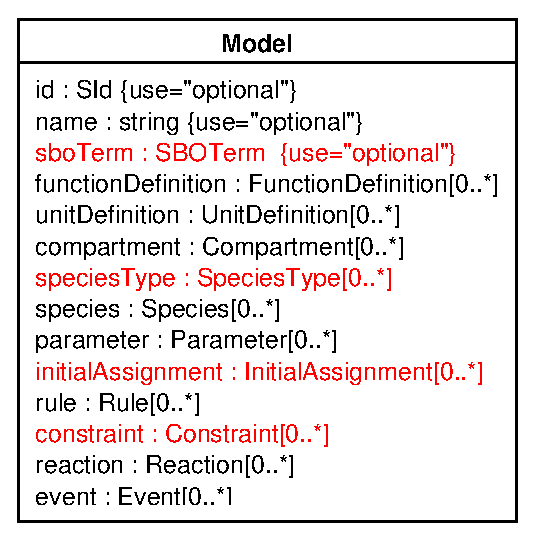
\includegraphics[scale = 0.65]{figs/model}
  \caption{The definition of \class{Model}.  Additional fields are
    inherited from \class{SBase}.}
  \vspace*{-0.7ex}
  \label{fig:model}
\end{figure}

\changed{\class{Model} serves as a container for \class{UnitDefinition},
  \class{Compartment}, \class{Species}, \class{Parameter}, \class{Rule},
  and \class{Reaction} components.  All of these components are optional;
  that is, the lists in each of the respective fields are permitted to have
  zero length.  (However, there are dependencies between components, such
  that defining some requires defining others.  See in particular
  Section~\ref{sec:species} on \class{Species}.)}  An instance of a
\class{Model} may also have an optional \attrib{name} field that can be
used to give the model a name.  The name must be a text string conforming
to the syntax permitted by the \class{SName} data type described in
Section~\ref{sec:name}.

In the XML encoding of an SBML model, the lists of species, compartments,
unit definitions, parameters, reactions, function definitions and rules
are translated into lists of XML elements that each have headings of the
form \class{listOf}\rule{0.5in}{0.5pt}\class{s}, where the blank is
replaced by the name of the component type (e.g., ``\texttt{Reaction}'').
The resulting XML data object has the form illustrated by the following
skeletal model:

\begin{example}
<?xml version="1.0" encoding="UTF-8"?>
<sbml xmlns="http://www.sbml.org/sbml/level1" level="1" version="\changed{2}">
  <model name="the_name_of_my_model">
    <listOfUnitDefinitions>
        ...
    </listOfUnitDefinitions>
    <listOfCompartments>
        ...
    </listOfCompartments>
    <listOfSpecies>
        ...
    </listOfSpecies>
    <listOfParameters>
        ...
    </listOfParameters>
    <listOfRules>
        ...
    </listOfRules>
    <listOfReactions>
        ...
    </listOfReactions>
  </model>
</sbml>
\end{example}

Readers may wonder about the motivations for the
\class{listOf}\rule{0.5in}{0.5pt}\class{s} notation.  A simpler approach to
creating the lists of components would be to place them all directly
at the top level under \texttt{<model> ... </model>}.  We chose instead to
group them within XML elements named after
\class{listOf}\rule{0.5in}{0.5pt}\class{s}, because we believe this helps
organize the components and makes visual reading of model definitions
easier.


%-----------------------------------------------------------------------------
\subsection{Unit Definitions}
\label{sec:unitdefinitions}
%-----------------------------------------------------------------------------

Units may be supplied in a number of contexts in an SBML model.  A facility
for defining units is convenient to have so that combinations of units can
be given abbreviated names.  This is the motivation behind the
\class{UnitDefinition} data structure, whose definition is shown in
Figure~\vref{fig:unitdefinition}.

\begin{figure}[htb]
  \centering
  
\includegraphics[scale = 0.65]{figs/unitdefinition}
  \vspace*{-4pt}
  \caption{The definition of \class{UnitDefinition}.}
  \label{fig:unitdefinition}
\end{figure}

A unit definition consists of a \attrib{name} field of type \class{SName}
and an optional list of structures of type \class{Unit}.  The approach to
defining units in SBML is compositional; for example, $meter\ 
second^{\,-2}$ is constructed by combining a \class{Unit}-type element
representing $meter$ with a \class{Unit}-type element representing
$second^{\,-2}$.  \changed{The \class{Unit} structure has one required
  attribute, \attrib{kind}, whose value must be a name taken from the list
  of units in Table~\ref{tab:unitkind}.  The optional \attrib{exponent}
  field on \class{Unit} represents an exponent on the unit.}  Its default
value is ``\attribvalue{1}'' (one).  In the example just mentioned,
$second^{\,-2}$ is obtained by using \texttt{kind="second"} and
\texttt{exponent="-2"}.  \changed{Finally, a \class{Unit} structure also
  has an optional \attrib{scale} field; its value must be an integer
  exponent on a power of ten multiplier used to set the scale of the unit.}
For example, a unit that has a \attrib{kind} value of ``\texttt{gram}'' and
a \attrib{scale} value of ``\texttt{-3}'' signifies $10^{-3} * gram$, or
milligrams.  \changed{The default value of \texttt{scale} is zero, because
  $10^0 = 1$.}

\begin{table}[thb]
  \centering
%  \vspace*{5pt}
  \ttfamily
  \begin{tabular}{llllll}
    \toprule
    ampere      	& farad	& joule		& lumen		& ohm     & steradian\\
    becquerel   	& gram	& katal		& lux		& pascal  & tesla\\
    candela		& gray	& kelvin	& meter		& radian  & volt\\
    celsius		& henry	& kilogram	& metre		& second  & watt\\
    coulomb		& hertz	& liter		& mole		& siemens & weber\\
    \underline{dimensionless} & \underline{item} & litre	& newton	& sievert\\
    \bottomrule
  \end{tabular}
  \caption{The possible values of \attrib{kind} in a \class{UnitKind}
    structure.  All are names of base or derived SI units, except for
    ``\texttt{dimensionless}'' and ``\texttt{item}'', which are 
    SBML additions important for handling certain common cases.
    ``\texttt{Dimensionless}'' is intended for cases where a quantity does not
    have units, and ``\texttt{item}'' is  needed in certain contexts to express
    such things as ``N items'' (e.g., ``100 molecules'').
    \changed{Although ``\texttt{Celsius}'' should be capitalized, for 
    simplicity SBML
    requires that all unit names be treated in a case-insensitive manner.}
    Also, note that the gram and liter/litre are not
    strictly part of SI~\protect\changed{\citep{bipm:2000}}; however, they
    are \changed{so commonly used in SBML's areas of application that they 
    are included as predefined unit names.}  (The standard SI unit of
    mass is in fact the kilogram, and volume is
    defined in terms of cubic meters.)}
  \label{tab:unitkind}
\end{table}

Unit combinations are constructed by listing several \class{Unit}
structures inside a \class{UnitDefinition}-type structure.  The following
example illustrates the definition of an abbreviation named
``\texttt{mmls}'' for the units $mmol\ l^{-1}\ s^{-1}$:

\begin{example}
<listOfUnitDefinitions>
    <unitDefinition name="mmls">
        <listOfUnits>
            <unit kind="mole"   scale="-3"/>
            <unit kind="liter"  exponent="-1"/>
            <unit kind="second" exponent="-1"/>
        </listOfUnits>                
    </unitDefinition>
</listOfUnitDefinitions>
\end{example}

\begin{blockChanged}
There are three special unit names in SBML, listed in
Table~\ref{tab:builtin}, corresponding to the three types of quantities
that play roles in biochemical reactions: amount of substance, volume and
time.  SBML defines default units for these quantities, all with a default
\texttt{scale} value of \texttt{0}.  The various components of a model,
such as parameters, can use only the predefined units from
Table~\ref{tab:unitkind}, new units defined in unit definitions, or the
three predefined names ``\texttt{substance}'', ``\texttt{time}'', and
``\texttt{volume}'' from Table~\ref{tab:builtin}.  The latter usage
signifies that the units to be used should be the designated defaults.  
\end{blockChanged}

\begin{table}[tb]
  \vspace*{-4pt}
  \centering
  \small
  \setlength{\tabcolsep}{4.5pt}
  \begin{blockChanged}
  \begin{tabular}{lllc}
    \toprule
    \textbf{Name} & \textbf{Allowable Units} & \textbf{Default Units}\\
    \midrule
    \texttt{substance} & moles \emph{or} number of molecules     & moles \\
    \texttt{volume}                & liters           & liters \\
    \texttt{time}                  & seconds          & seconds \\
    \bottomrule
  \end{tabular}
  \end{blockChanged}
  \caption{SBML's built-in quantities.  Each of these units has a default
  \texttt{scale} value of \texttt{0}.}
  \label{tab:builtin}
\end{table}

\begin{blockChanged}
A model may change the default scales by reassigning the special unit names
``\texttt{substance}'', ``\texttt{time}'', and ``\texttt{volume}'' in a
unit definition.  This takes advantage of the \class{UnitDefinition}
structure's facility for defining scales on units.  The following example
changes the default units of volume to be milliliters:
\end{blockChanged}

\begin{example}
<model>
    ...
    <listOfUnitDefinitions>
        <unitDefinition name="volume">
            <listOfUnits>
                <unit kind="liters" scale="-3"/>
            </listOfUnits>                
        </unitDefinition>
    </listOfUnitDefinitions>
    ...
</model>
\end{example}

If the definition above appeared in a model, the volume scale on all
components that did not explicitly use different units would be changed to
milliliters.  


%-----------------------------------------------------------------------------
\subsection{Compartments}
\label{sec:compartments}
%-----------------------------------------------------------------------------

A \emph{compartment} in SBML represents a bounded volume in which species
are located.  Compartments do not necessarily have to correspond to actual
structures inside or outside of a cell, although models are often designed
that way.  The definition of \class{Compartment} is shown in
Figure~\vref{fig:compartment}.

\begin{figure}[htb]
  \vspace*{1pt}
  \centering
  
\includegraphics[scale = 0.65]{figs/compartment}
  \vspace*{-3pt}
  \caption{The definition of \class{Compartment}.  
    Fields inherited from \class{SBase} are omitted here but are assumed.}
  \label{fig:compartment}
\end{figure}

\begin{blockChanged}
\class{Compartment} has one required field,
\attrib{name}, to give it a unique name by which other parts of an SBML
model definition can refer to it.  A compartment can also have an optional
floating-point field called \attrib{volume} representing the total volume
of the compartment.  This enables concentrations of species to be
calculated in the absence of spatial geometry information.%
\end{blockChanged}
The \attrib{volume} attribute defaults to a value of ``\texttt{1}'' (one).
\begin{blockChanged}
The units of volume may be explicitly set using the optional field
\attrib{units}.  The value of this attribute must be one of the following:
a predefined unit name from Table~\ref{tab:unitkind}, the term
``\attrib{volume}'' (which, if used, signifies that the default units of
volume should be used---see Section~\ref{sec:unitdefinitions}), or the
name of a unit defined by a unit definition in the 
\class{Model}.  If absent, as in the example above, the units default to
the value set by the built-in ``\attrib{volume}''.\end{blockChanged}

The optional field \attrib{outside} of type \class{SName} can be used to
express containment relationships between compartments.  If present, the
value of \attrib{outside} for a given compartment
\begin{blockChanged}
must be the name of
another compartment enclosing it, or in other words, the compartment that
is ``outside'' of it.  This enables the representation of simple
topological relationships between compartments, for those simulation
systems that can make use of the information (e.g., for drawing simple
diagrams of compartments).  Although containment relationships are partly
taken into account by the compartmental localization of reactants and
products, it is not always
\end{blockChanged}
\begin{blockChanged} possible to determine purely from the reaction
equations whether one compartment is meant to be located within another.
In the absence of a value for \attrib{outside}, compartment definitions in
SBML Level~1 do not have any implied spatial relationships between each
other.
\end{blockChanged}

In an XML data stream containing an SBML model, compartments are listed
inside an XML element called \attrib{listOfCompartments} within a
\class{Model}-type data structure.  (See the discussion of \class{Model} in
Section~\ref{sec:model}.)  The following example illustrates two
compartments in an abbreviated SBML example of a model definition:
\begin{example}
<model>
    ...
    <listOfCompartments>
        <compartment name="cytosol" volume="2.5"/>
        <compartment name="mitochondria" volume="0.3"/>
    </listOfCompartments>
    ...
</model>
\end{example}

\begin{blockChanged}
The following is an example of using \attrib{outside} to model a cell
membrane.  To express that a compartment named B has a membrane that is
modeled as another compartment M, which in turn is located within another
compartment A, one would write:
\end{blockChanged}
\begin{example}
<model>
    ...
    <listOfCompartments>
        <compartment name="A"/>
        <compartment name="M" outside="A"/>
        <compartment name="B" outside="M"/>
    </listOfCompartments>
    ...
</model>
\end{example}


%-----------------------------------------------------------------------------
\subsection{Species}
\label{sec:species}
%-----------------------------------------------------------------------------

The term \emph{species} refers to entities that take part in reactions.
These include simple ions (e.g., protons, calcium), simple molecules (e.g.,
glucose, ATP), and large molecules (e.g., RNA, polysaccharides, and
proteins).  The \class{Species} data structure is intended to represent
these entities.  Its definition is shown in Figure~\vref{fig:species}.

\begin{figure}[htb]
  \centering
  \vspace*{5pt}
  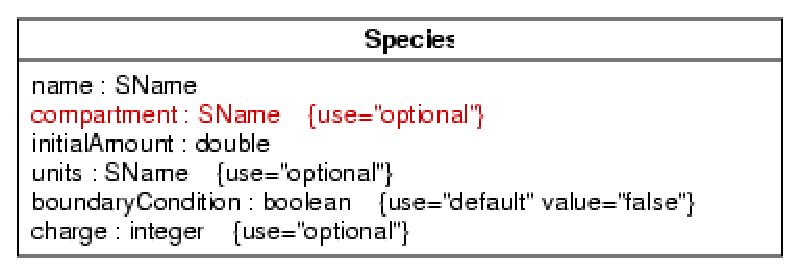
\includegraphics[scale = 0.65]{figs/species}
  \caption{The definition of \class{Species}.  As usual, fields inherited from
    \class{SBase} are omitted here but are assumed.}
  \label{fig:species}
\end{figure}

\class{Species} has a required \attrib{name} field of type \class{SName}.
The required field \attrib{compartment}, also of type \class{SName}, is
used to identify the compartment in which the species is located.  The field
\attrib{initialAmount}, of type \class{double}, is used to set the initial
amount of the species in the named compartment.  The units of \changed{this
  quantity may be set explicitly using the optional field \attrib{units}.
  The value of \attrib{units} must be chosen from one of the following
  possibilities: a predefined unit name from Table~\ref{tab:unitkind}, the
  term ``\texttt{substance}'' (which, if present, signifies that the
  default} \changed{units of quantity should be used---see
  Section~\ref{sec:unitdefinitions}), or a new unit name defined by a unit
  definition in the enclosing \class{Model}.  If absent, the units default
  to the value set by the built-in ``\texttt{substance}''.}

The optional boolean field \attrib{boundaryCondition} determines whether
the amount of the \changed{species} is fixed or variable over the course of
a simulation.  The value of \attrib{boundaryCondition} defaults to
``\texttt{false}'', indicating that by default, the amount is not fixed.
\changed{If the amount of a species is defined as being fixed, it
implies that some external mechanism maintains a constant quantity in the
compartment throughout the course of a reaction.  (The term \emph{boundary
  condition} alludes to the role of this constraint in a simulation.)}

The optional field \attrib{charge} is an integer indicating the charge on
the species (in terms of electrons, not the SI unit Coulombs).  This may be
useful when the \changed{species} involved is a charged ion such as calcium
(\changed{$\text{Ca}^{2+}$}).

The following example shows two \changed{species} definitions within an
abbreviated SBML model definition.  The example shows that species are
listed under the heading \attrib{listOfSpecies} in the model:
\begin{example}
<model>
    ...
    <listOfSpecies>
        <species name="Glucose" compartment="cell" initialAmount="4"/>
        <species name="Glucose_6_P" compartment="cell" initialAmount="0.75"/>
    </listOfSpecies>
    ...
</model>
\end{example}

%Note that the compartment's name is used instead of an identifier, because
%simulation systems typically enable users to locate species using
%compartment names rather than machine-generated identifiers.  Since a
%compartment's name must be unique among all the compartments in a model
%(see the discussion of namespaces in Section~\ref{sec:namespaces}), there
%is no danger of ambiguity and no compelling reason to introduce identifiers
%on compartments.

\begin{blockChanged}
  In SBML Level 1 Version~2, the term \emph{specie} (used in SBML Level~1
  Version~1) has been replaced with the more commonly-accepted spelling
  \emph{species} throughout the specification.  Models written in SBML
  Level~1 Version~2 format should use the new spelling.  However, for
  backwards compatibility, software packages intended to be conformant with
  SBML Level~1 Version~2 should accept \emph{both} spellings on input for
  all elements and attributes where the term occurs.  Beginning with SBML
  Level~2, the \emph{specie} spelling will be removed entirely and only
  \emph{species} will be used.
\end{blockChanged}

\begin{blockChanged}
  Finally, note that the definition of \class{Species} in SBML requires a
  species in a model to be located within a compartment.  This means that
  at least one compartment must be defined in an SBML model that defines
  any species.  The only exception to this is the case of degenerate models
  that have no species or reactions.
\end{blockChanged}

\vspace*{1ex}                           % HACK TO GET BETTER PAGE SPACING

%-----------------------------------------------------------------------------
\subsection{Parameters}
\label{sec:parameters}
%-----------------------------------------------------------------------------

A \class{Parameter} structure is used to associate a \changed{name} with a
floating-point value so that the symbol can be used in formulas in place of
the value.  The definition of \class{Parameter} is shown in
Figure~\vref{fig:parameter}.

\begin{figure}[htb]
  \centering
  \vspace*{8pt}
  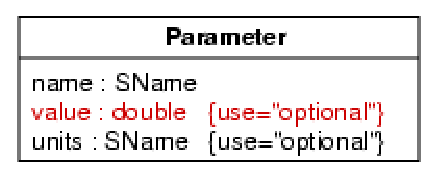
\includegraphics[scale = 0.65]{figs/parameter}
  \caption{The definition of \class{Parameter}.}
  \label{fig:parameter}
\end{figure}

\changed{The \class{Parameter} structure has one required field,
  \attrib{name}, representing the parameter's name in the model.}  The
\changed{optional} field \attrib{value} determines the value (of type
\class{double}) assigned to the symbol.  The units of the parameter
\attrib{value} are specified by the field \attrib{units}.  The value
assigned to \attrib{units} must be chosen from one of the following
possibilities: one of \changed{the} base unit names from
Table~\vref{tab:unitkind}; one of the three names
``\attribvalue{substance}'', ``\attribvalue{time}'', or ``\attrib{volume}''
(see Table~\ref{tab:builtin}); or the name of a new unit defined in the
list of unit definitions in the enclosing \class{Model} structure.

Parameters \changed{can be defined} in two places in SBML: in lists of
parameters defined at the top level in a \class{Model}-type structure
\changed{(in the \class{listOfParameters} described in
  Section~\ref{sec:model})}, and within individual reaction definitions
\changed{(as described in Section~\ref{sec:reactions})}.  Parameters
defined at the top level are \emph{global} to the whole model; parameters
that are defined within a reaction are local to the particular reaction and
(within that reaction) \emph{override} any global parameters having the
same names.  (See Section~\ref{sec:namespaces} for further details.)

\clearpage                           % HACK TO GET BETTER PAGE SPACING

The following is an example of parameters defined at the \class{Model} level:

\begin{example}
<model>
    ...
    <listOfSpecies>
        ...
    </listOfSpecies>
    <listOfParameters>
        <parameter name="Km1" value="2.3" units="second"/>
        <parameter name="Km2" value="10.7" units="second"/>
    </listOfParameters>
    <listOfReactions>
        ...
    </listOfReactions>
    ...
</model>
\end{example}

An example of a full model that uses parameters is presented in
Section~\ref{subsection:ruleseg}.


%-----------------------------------------------------------------------------
\subsection{Rules}
\label{sec:rules}
%-----------------------------------------------------------------------------

In SBML, \emph{rules} provide a way to create constraints on variables for
cases in which the constraints cannot be expressed using \changed{reactions
  (Section~\ref{sec:reactions}) nor the assignment of an initial value to a
  component in a model}.  There are two orthogonal dimensions by which
rules can be described.  First, there are three different possible
functional forms, corresponding to the following three general cases
\changed{(where $x$ is a variable, $f$ is some arbitrary function, and $W$
  is a vector of parameters and variables that may include $x$):}

\begin{blockChanged}
\begin{center}
\begin{tabular}{rll}
(Algebraic rule) & left-hand side is zero:             & $0 = f(W)$\\
(Scalar rule) 	& left-hand side is a scalar:         & $x = f(W)$\\
(Rate rule) 	& left-hand side is a rate-of-change: & $dx/dt = f(W)$
\end{tabular}
\end{center}
\end{blockChanged}

The second dimension concerns the role of variable $x$ in the equations
above: $x$ can be the name of a compartment (to set its volume), the name
of a \changed{species} (to set its concentration), or a parameter name (to
set its value).  

\begin{blockChanged}
In their general form given above, there is little to distinguish between
scalar and algebraic rules.  They are treated as separate cases for the
following reasons:
\begin{itemize}
  
\item Scalar rules can simply be evaluated to calculate intermediate
  values for use in numerical methods.
  
\item Some simulators do not contain numerical solvers capable of solving
  unconstrained algebraic equations.
  
\item Those simulators that \emph{can} solve algebraic equations normally
  make a distinction between the different categories listed above;
  therefore, it is important to distinguish them also in a model
  definition.
  
\item Some specialized numeric analyses of models may only be applicable to
  models that do not contain algebraic rules; therefore, it is important to
  indicate the presence of such rules in a model.
\end{itemize}
\end{blockChanged}

The approach taken to covering these cases in SBML is to define an abstract
\class{Rule} structure that contains just one field, \attrib{formula}, to
hold the right-hand side expression, then to derive subtypes of
\class{Rule} that add fields to cover the various cases above.
Figure~\vref{fig:rules} gives the definitions of \class{Rule} and the
subtypes derived from it.  The figure shows that \class{AlgebraicRule} is
defined directly from \class{Rule}, whereas \class{CompartmentVolumeRule},
\class{SpeciesConcentrationRule}, and \class{ParameterRule} are all derived
from an intermediate abstract structure called \class{AssignmentRule}.

\begin{figure}[htb]
  \centering
  \vspace*{-3pt}
  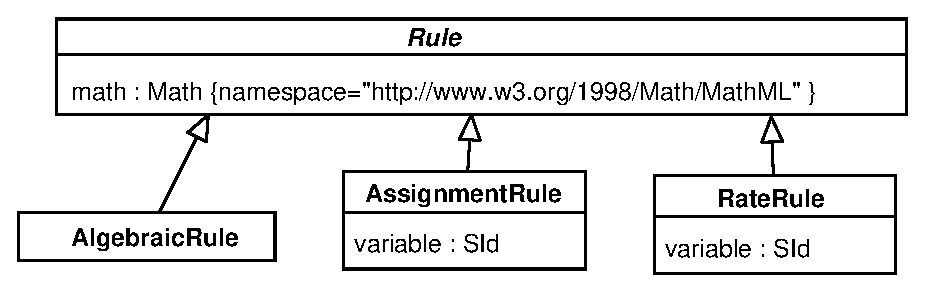
\includegraphics[scale = 0.65]{figs/rule}
  \vspace*{-3pt}
  \caption{The definition of \class{Rule} and derived types.}
  \label{fig:rules}
\end{figure}

The \attrib{type} field introduced in \class{AssignmentRule} is an
enumeration of type \class{RuleType} that determines whether a rule falls
into the \changed{scalar or rate categories} in the list of cases above.
In SBML Level~1, the enumeration has two possible values:
``\class{scalar}'' and ``\class{rate}''.  The former means that the
expression has a scalar value on the left-hand side [i.e., \changed{$x =
  f(W)$}, as in case 2 in the list above]; the latter means that the
expression has a rate of change differential on the left-hand side
\changed{[i.e., $dx/dt = f(X)$, as in case 3 in the list above]}.  Future
releases of SBML may add to the possible values of \class{RuleType}.


\subsubsection{\class{AlgebraicRule}}

The rule type \class{AlgebraicRule} is used to express equations whose
left-hand sides are zero.  \class{AlgebraicRule} does not add any fields to
the basic \class{Rule}; its role is simply to distinguish this case from
the other cases.


\subsubsection{\class{SpeciesConcentrationRule}}

The \class{SpeciesConcentrationRule} structure adds one field,
\changed{\attrib{species}}, to the basic \class{AssignmentRule} type.  The
field \changed{\attrib{species}} has type \class{SName} and is used to
identify the \changed{species} affected by the rule.  The effect of the
rule depends on the value of \attrib{type}: if the value is
``\class{scalar}'', the rule sets the referenced \changed{species}'
concentration to the value determined by the formula; if the value is
``\class{rate}'', the rule sets the rate of change of the \changed{species}'
concentration to the value determined by the formula.  The units are in
terms of $substance/volume$, where the $substance$ units are those that are
declared on the referenced \class{Species} element, and the $volume$ units
are those declared on the \class{compartment} element that contains the
\class{Species}.

\begin{blockChanged}
  Unless the \attrib{boundaryCondition} field of a given species is set to
  ``\attribvalue{true}'', that species cannot be named by both a
  \class{SpeciesConcentrationRule} structure and a \class{SpeciesReference}
  structure (see Section~\ref{sec:reactions}).  This restriction simply
  codifies the notion that it would be a logical inconsistency to define a
  rule for a species whose concentration is already being altered by one or
  more reactions.
\end{blockChanged}


\subsubsection{\class{CompartmentVolumeRule}}

The \class{CompartmentRule} structure adds one field, \attrib{compartment},
to the basic \class{AssignmentRule} type.  The field \attrib{compartment}
has type \class{SName} and is used to identify the compartment affected by
the assignment.  The effect of the rule depends on the value of
\attrib{type}: if the type is ``\class{scalar}'', the rule sets the
referenced compartment's volume to the volume determined by the formula; if
the type is ``\class{rate}'', the rule sets the rate of change of the
compartment's volume to the volume determined by the formula.
\changed{No more than one \class{CompartmentVolumeRule} can refer to a
given compartment in an SBML model definition.}


\subsubsection{\class{ParameterRule}}
\label{sec:parameterrule}

The \class{ParameterRule} structure adds two fields, \attrib{name} and
\attrib{units}, to the basic \class{AssignmentRule} type.  The
\attrib{name} attribute has type \class{SName} and identifies the
parameter.  \changed{The parameter must already exist and be defined by a
  \class{Parameter} structure in the enclosing model; in other words,
  \class{ParameterRule} does not create new symbols.}  The \attrib{units}
field acts in the same way as in the case of the \class{Parameter}
structure (Section~\ref{sec:parameters}).  The value assigned to
\attrib{units} must be chosen from one of the following possibilities: one
of base unit names from table~\ref{tab:unitkind}; one of the three names
``\attribvalue{substance}'', ``\attribvalue{time}'', or ``\attrib{volume}''
(see Table~\ref{tab:builtin}); or the name of a new unit defined in the
list of unit definitions in the enclosing \class{model} structure.

The effect of this rule depends on the value of the \attrib{type} field in
\class{AssignmentRule}: if the type is ``\texttt{scalar}'', the rule sets
the referenced parameter's value to that determined by the formula in
\attrib{math}; if the type is ``\texttt{rate}'', the rule sets the rate of
change of the parameter's value to that determined by the formula.

\subsubsection{Constraints on Rule Use}
\label{sec:ruleconstraints}

\begin{blockChanged}
SBML specifically does not stipulate the form of the algorithms that can be
applied to rules and reactions.  For example, SBML does not specify when or
how often rules should be evaluated.  The constraints described by rules
and kinetic rate laws are meant to apply collectively to the set of
variable values for a specific time.

To prevent ambiguities and inconsistencies in an SBML model, no more than
one assignment rule can be defined for a given identifier.  A
\texttt{scalar} rule for a given identifier overrides the initial value of
that identifier; i.e., the initial value should be ignored.  This does not
mean that any structure declaring an identifier can be omitted if there is
a \texttt{scalar} rule for that identifier.  For example, there must be a
\texttt{Parameter} structure for a given parameter if there is a
\texttt{ParameterRule} for that parameter.

The ordering of \texttt{scalar} rules is significant: they are always
evaluated in the order given in SBML.  The \attrib{formula} field of a
\texttt{scalar} rule structure can contain any identifier except for the
following: (a) identifiers for which there exists a subsequent
\texttt{scalar} rule, and (b) the identifier for which the rule is defined.
These constraints are designed to eliminate algebraic loops among the
scalar rules.  Eliminating algebraic loops ensures that scalar rules can be
evaluated any number of times in a simulation without the result of those
evaluations changing.

As an example of all this, consider the following equations, in the order
shown:
\begin{equation*}
  \begin{array}{lll}
    x = x + 1, & y = z + 200, & z = y + 100
  \end{array}
\end{equation*}
If this set of equations were interpreted as a set of scalar rules, it
would be invalid because the rule for $x$ refers to $x$ and the rule for
$y$ refers to $z$ before $z$ is defined.
\end{blockChanged}


\subsubsection{Example of Rule Use}

The following is an example use of rules:

\begin{example}
<model>
    ...
    <listOfRules>
        <parameterRule name="k" formula="k3/k2"/>
        <speciesConcentrationRule species="s2" formula="k * z/(1 + k)"/>
        <compartmentVolumeRule compartment="A" formula="0.10 * k4"/>
    </listOfRules>
    ...
</model> 
\end{example}


%-----------------------------------------------------------------------------
\subsection{Reactions}
\label{sec:reactions}
%-----------------------------------------------------------------------------

A \emph{reaction} represents some transformation, transport or binding
process, typically a chemical reaction, that can change the amount of one
or more species.  The \class{Reaction} type is defined in
Figure~\ref{fig:reaction}.  

\begin{figure}[htb]
  \centering
  \vspace*{8pt}
  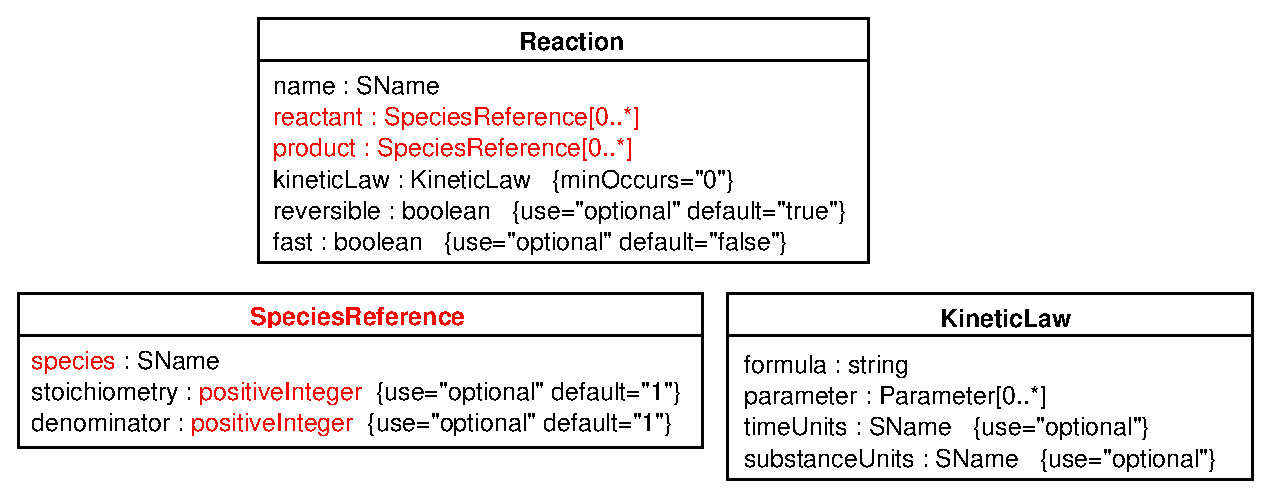
\includegraphics[scale = 0.65]{figs/reaction}
  \caption{The definitions of \class{Reaction}, \class{KineticLaw} and
    \changed{\class{SpeciesReference}}.} 
  \label{fig:reaction}
\end{figure}

In SBML, reactions are defined using lists of reactant species, products,
and their stoichiometries, and by parameter values for separately-defined
kinetic laws.  These various quantities are recorded in the fields
\attrib{reactant}, \attrib{product}, and \attrib{kineticLaw}.  Both
\attrib{reactant} and \attrib{product} are references to species
implemented using lists of \changed{\class{SpeciesReference}} structures
(defined in Section~\ref{subsec:speciesreference} below).  The
\changed{\class{SpeciesReference}} structure contains fields for recording
the names of species and their stoichiometries.  \attrib{kineticLaw} is an
optional field of type \class{KineticLaw} (defined in
Section~\ref{subsec:kinetic-law} below), used to provide a mathematical
formula describing the rate of the reaction.

In addition to these fields, the \class{Reaction} structure also has a
boolean field, \attrib{reversible}, that indicates whether the reaction is
reversible.  The field is optional, and if left unspecified in a model, it
defaults to a value of ``\attribvalue{true}''.  Information about
reversibility is useful in certain kinds of structural analyses such as
elementary mode analysis.

The field \attrib{fast} is another boolean attribute in the
\class{Reaction} data structure; a value of ``\attribvalue{true}''
signifies that the given reaction is a ``fast'' one.  This may be relevant
when computing equilibrium concentrations of rapidly equilibrating
reactions.  Simulation/analysis packages may \changed{choose} to use this
information to reduce the number of ODEs required and thereby optimize such
computations.  The default value of \attrib{fast} is
``\attribvalue{false}''.  (A simulator/analysis package that has no
facilities for dealing with fast reactions can ignore this attribute.  In
theory, if the choice of which reactions are fast is correctly made, then a
simulation performed with them should give the same results as a simulation
performed without fast reactions.  However, currently there appears to be
no single unambiguous method for designating which reactions should be
considered fast, and some users may designate a reaction as fast when in
fact it is not.  Caveat developer.)


\subsubsection{\changed{\class{SpeciesReference}}}
\label{subsec:speciesreference}

Each unique \changed{species} involved in a reaction is listed once in a
model, in a list contained in the \changed{\attrib{species}} field of the
\class{Model} data structure discussed in Section~\ref{sec:model}.  Lists
of products and reactants in \class{Reaction} type structures refer to
those species.  The connection between the products and reactants in a
reaction definition and the \changed{species} names listed in the enclosing
\class{Model} definition is achieved using the
\changed{\class{SpeciesReference}} type data structure defined in
Figure~\vref{fig:reaction}.

The field \changed{\attrib{species}} of type \class{SName} in
\changed{\class{SpeciesReference}} must refer to the name of a
\changed{species} defined in the enclosing \class{Model}-type structure.
The two fields \attrib{stoichiometry} and \attrib{denominator} together set
the stoichiometry value for a \changed{species} in a reaction.  Both
\changed{take positive integers as values}, and both have default values of
``\attribvalue{1}'' (one).  \changed{The absolute value of the
  stoichiometric number is the value of \attrib{stoichiometry} divided by
  \attrib{denominator}, and the sign is implicit from the role of the
  species (i.e., positive for reactants and negative for products).}  The
use of these separate terms allows a simulator to employ rational
arithmetic on the stoichiometry matrix \changed{if it is capable of it},
potentially reducing round-off errors and other problems during
computations.  Such computations are particularly important when working
with large matrices and calculating such things as elementary modes.

The following is a simple example of a \changed{species} reference in a
list of reactants within a reaction named ``J1'':
\begin{example}
<model>
    ...
    <listOfReactions>
        <reaction name="J1">
            <listOfReactants>
                <\changed{speciesReference} \changed{species}="X0" stoichiometry="2"/>
            </listOfReactants>
            ...
        </reaction>
        ...
    </listOfReactions>
    ...
</model>
\end{example}

\subsubsection{\class{KineticLaw}}
\label{subsec:kinetic-law}

A \class{kineticLaw} structure describes the rate of the enclosing
reaction.  The use of a \class{KineticLaw} structure in a \class{Reaction}
component is optional.  (\changed{In general, there is no useful default
  value that can be substituted in place of a missing kinetic law, but the
  element is optional because certain kinds of network analysis are still
  possible in the absence of information on reaction kinetics.})

The field \attrib{formula}, of type \class{string}, expresses the rate in
$substance/time$ units.  (Section~\ref{sec:formulas} discusses formulas.)
The optional fields \attrib{substanceUnits} and \attrib{timeUnits}
determine the units of substance and time.  If not set, the units are taken
from the defaults defined by the built-in ``\texttt{substance}'' and
``\texttt{time}'' of Table~\vref{tab:builtin}.

A \class{KineticLaw} type structure can contain zero or more
\class{Parameter} structures (Section~\ref{sec:parameters}) that define
symbols that can be used in the \attrib{formula} string.  As discussed in
Section~\ref{sec:namespaces}, reactions introduce local namespaces for
parameter names.  Within a \class{KineticLaw} structure inside a reaction
definition, a parameter whose name is identical to a global parameter
defined in the enclosing \class{Model}-type structure takes precedence over
that global parameter.

The following is an example of a \class{Reaction} structure that defines
the reaction $J_1: \ X_0 \longrightarrow S_1; \ k_1 X_0$.  It demonstrates
the use of \changed{species} references and the \class{KineticLaw}
structure:
\begin{example}
<model>
    ...
    <listOfReactions>
        <reaction name="J1">
            <listOfReactants>
                <\changed{speciesReference} \changed{species}="X0" stoichiometry="1"/>
            </listOfReactants>
            <listOfProducts>
                <\changed{speciesReference} \changed{species}="S1" stoichiometry="1"/>
            </listOfProducts>
            <kineticLaw formula="k1*X0">
                <listOfParameters>
                    <parameter name="k1" value="0"/>
                </listOfParameters>
            </kineticLaw>
        </reaction>
    </listOfReactions>
    ...
</model>
\end{example}


%=============================================================================
\section{Examples of Full Models Encoded in XML Using SBML}
\label{sec:xml-rep}
%=============================================================================

In this section, we present several examples of complete models encoded in
XML using SBML Level~1.  Our approach to translating the UML-based
structure definitions presented in the previous sections is described
elsewhere~\citep{hucka:2000b}.  Appendix~\ref{apdx:schemas} gives the full
listing of an XML Schema corresponding to SBML Level~1.


%-----------------------------------------------------------------------------
\subsection{A Simple Example Application of SBML}
%-----------------------------------------------------------------------------

Consider the following hypothetical branched system:
\begin{equation*}
  \begin{array}{@{}ccc@{}}
    X_0 & \underrightarrow{k_1 X_0} & S_1 \\ \\[-4pt]
    S_1 & \underrightarrow{k_2 S_1} & X_1 \\ \\[-4pt]
    S_1 & \underrightarrow{k_3 S_1} & X_2
  \end{array}
\end{equation*}

The following is the main portion of an XML document that encodes the model
shown above:

\clearpage


\begin{example}
<?xml version="1.0" encoding="UTF-8"?>
<sbml xmlns="http://www.sbml.org/sbml/level1" level="1" version="\changed{2}">
    <model name="Branch">
        <notes>
            <body xmlns="http://www.w3.org/1999/xhtml">
                <p>Simple branch system.</p>
                <p>The reaction looks like this:</p>
                <p>reaction-1:   X0 -> S1; k1*X0;</p>
                <p>reaction-2:   S1 -> X1; k2*S1;</p>
                <p>reaction-3:   S1 -> X2; k3*S1;</p>
            </body>
        </notes>
        <listOfCompartments>
            <compartment name="compartmentOne" volume="1"/>
        </listOfCompartments>
        <listOfSpecies>
            <\changed{species} name="S1" initialAmount="0" compartment="compartmentOne"
                     boundaryCondition="false"/>
            <\changed{species} name="X0" initialAmount="0" compartment="compartmentOne"
                     boundaryCondition="true"/>
            <\changed{species} name="X1" initialAmount="0" compartment="compartmentOne"
                     boundaryCondition="true"/>
            <\changed{species} name="X2" initialAmount="0" compartment="compartmentOne"
                     boundaryCondition="true"/>
        </listOfSpecies>
        <listOfReactions>
            <reaction name="reaction_1" reversible="false">
                <listOfReactants>
                    <\changed{speciesReference} \changed{species=}"X0" stoichiometry="1"/>
                </listOfReactants>
                <listOfProducts>
                    <\changed{speciesReference} \changed{species=}"S1" stoichiometry="1"/>
                </listOfProducts>
                <kineticLaw formula="k1 * X0">
                    <listOfParameters>
                        <parameter name="k1" value="0"/>
                    </listOfParameters>
                </kineticLaw>
            </reaction>
            <reaction name="reaction_2" reversible="false">
                <listOfReactants>
                    <\changed{speciesReference} \changed{species=}"S1" stoichiometry="1"/>
                </listOfReactants>
                <listOfProducts>
                    <\changed{speciesReference} \changed{species=}"X1" stoichiometry="1"/>
                </listOfProducts>
                <kineticLaw formula="k2 * S1">
                    <listOfParameters>
                        <parameter name="k2" value="0"/>
                    </listOfParameters>
                </kineticLaw>
            </reaction>
            <reaction name="reaction_3" reversible="false">
                <listOfReactants>
                    <\changed{speciesReference} \changed{species=}"S1" stoichiometry="1"/>
                </listOfReactants>
                <listOfProducts>
                    <\changed{speciesReference} \changed{species=}"X2" stoichiometry="1"/>
                </listOfProducts>
                <kineticLaw formula="k3 * S1">
                    <listOfParameters>
                        <parameter name="k3" value="0"/>
                    </listOfParameters>
                </kineticLaw>
            </reaction>
        </listOfReactions>
    </model>
</sbml>
\end{example}


\begin{blockChanged}
The XML encoding shown above is quite straightforward. The outermost
container is a tag, \texttt{<smbl>}, that identifies the contents as being
\underline{S}ystems \underline{B}iology \underline{M}arkup
\underline{L}anguage.  The first attribute, \attrib{xmlns}, is required for
tools that read XML to be able to verify the syntax of a given definition
against the XML Schema for SBML.  The attributes \texttt{level} and
\texttt{version} indicate that the content is formatted according to
Version~2 of the Level~1 definition of SBML.
\end{blockChanged}

The next-inner container is a single \texttt{<model>} element that serves
as the highest-level object in the model.  The model has a name,
``Branch''.  The model contains one compartment, four species, and three
reactions.  The elements in the \texttt{<listOfReactants>} and
\texttt{<listOfProducts>} in each reaction refer to the names of elements
listed in the \texttt{<listOfSpecies>}.  The correspondences between the
various elements is explicitly stated by the
\changed{\texttt{<speciesReference>}} elements.

The model includes a \texttt{<notes>} annotation that summarizes the model
in text form, with formatting based on XHTML.  This may be useful for a
software package that is able to read such annotations and, for example,
render them in HTML in a graphical user interface.


%-----------------------------------------------------------------------------
\subsection{Simple Use of Units Feature in a Model}
\label{apdx:units-eg}
%-----------------------------------------------------------------------------

The following model uses the units features of SBML Level~1.  In this
model, the default value of \texttt{substance} is changed in the list of
unit definitions to be mole units with a scale factor of $-3$, or
millimoles.  This sets the default substance units in the model,
\changed{although} components can override this scale locally.  The
\attrib{volume} and \attrib{time} built-ins are left to their defaults,
ensuring that volume is in liters and time is in seconds.  The result is
that, in this model, kinetic law formulas define rates in millimoles per
second and the \changed{species} symbols in them represent concentration
values in millimoles per liter.  All the \changed{\class{species}} elements
set the initial amount of every given \changed{species} to $1$ millimole.
The parameters \texttt{Vm} and \texttt{Km} are defined to be in millimoles
per liter per second, and milliMolar, respectively.

\begin{example}
<?xml version="1.0" encoding="UTF-8"?>
<sbml xmlns="http://www.sbml.org/sbml/level1" level="1" version="\changed{2}">
    <model>
        <listOfUnitDefinitions>
            <unitDefinition name="substance">
                <listOfUnits>
                    <unit kind="mole" scale="-3"/>
                </listOfUnits>
            </unitDefinition>
            <unitDefinition name="mls">
                <listOfUnits>
                    <unit kind="mole"   scale="-3"/>
                    <unit kind="liter"  exponent="-1"/>
                    <unit kind="second" exponent="-1"/>
                </listOfUnits>
            </unitDefinition>
        </listOfUnitDefinitions>
        <listOfCompartments>
            <compartment name="cell"/>
        </listOfCompartments>
        <listOfSpecies>
            <\changed{species} name="x0" compartment="cell" initialAmount="1"/>
            <\changed{species} name="x1" compartment="cell" initialAmount="1"/>
            <\changed{species} name="s1" compartment="cell" initialAmount="1"/>
            <\changed{species} name="s2" compartment="cell" initialAmount="1"/>
        </listOfSpecies>
        <listOfParameters>
            <parameter name="vm" value="2" units="mls"/>
            <parameter name="km" value="2"/>
        </listOfParameters>
        <listOfReactions>
            <reaction name="v1">
                <listOfReactants>
                    <\changed{speciesReference} \changed{species=}"x0"/>
                </listOfReactants>
                <listOfProducts>
                    <\changed{speciesReference} \changed{species=}"s1"/>
                </listOfProducts>
                <kineticLaw formula="(vm * s1)/(km + s1)"/>
            </reaction>
            <reaction name="v2">
                <listOfReactants>
                    <\changed{speciesReference} \changed{species=}"s1"/>
                </listOfReactants>
                <listOfProducts>
                    <\changed{speciesReference} \changed{species=}"s2"/>
                </listOfProducts>
                <kineticLaw formula="(vm * s2)/(km + s2)"/>
            </reaction>
            <reaction name="v3">
                <listOfReactants>
                    <\changed{speciesReference} \changed{species=}"s2"/>
                </listOfReactants>
                <listOfProducts>
                    <\changed{speciesReference} \changed{species=}"x1"/>
                </listOfProducts>
                <kineticLaw formula="(vm * s1)/(km + s1)"/>
            </reaction>
        </listOfReactions>
    </model>
</sbml>
\end{example}


%-----------------------------------------------------------------------------
\subsection{\changed{An Example of Using Rules}}
\label{subsection:ruleseg}
%-----------------------------------------------------------------------------

\begin{blockChanged}
This section contains a model which simulates a system containing
a fast reaction. This model uses rules to express the mathematics
of the fast reaction explicitly rather than using the implicit
\attrib{fast} field on a reaction element.  The system modeled is

\begin{equation*}
  \begin{array}{@{}ccc@{}}
    X_0 & \underrightarrow{k_1 X_0} & S_1 \\ \\[-4pt]
    S_1 & \underrightarrow{k_f S_1 - k_r S_2} & S_2 \\ \\[-4pt]
    S_2 & \underrightarrow{k_2 S_1} & X_1\\ \\[-4pt]
  \end{array}
\end{equation*}
\begin{equation*}
  \begin{array}{lllll}
    k_1 = 0.1, & k_2 = 0.15, & k_f = K_{eq} 10000, & k_r = 10000, & K_{eq}
    = 2.5.\\ \\[-4pt]
  \end{array}
\end{equation*}

This can be approximated with the following system:
\begin{equation*}
  \begin{array}{@{}ccc@{}}
    X_0 & \underrightarrow{k_1 X_0} & T \\ \\[-4pt]
    T & \underrightarrow{k_2 S_1} & X_1\\ \\[-4pt]
  \end{array}
\end{equation*}
\begin{equation*}
  \begin{array}{ll}
    S_1 = \D\frac{T}{1 + K_{eq}}, & S_2 = K_{eq} S_1\\ \\[-4pt]
  \end{array}
\end{equation*}

\changed{The following SBML example encodes the approximate form.}

\begin{example}
<?xml version="1.0" encoding="UTF-8"?>
<sbml xmlns="http://www.sbml.org/sbml/level1" level="1" version="\changed{2}">
    <model>
        <listOfCompartments>
            <compartment name="cell" volume="1"/>
        </listOfCompartments>
        <listOfSpecies>
            <species id="X0" compartment="cell" initialAmount="1"/>
            <species id="X1" compartment="cell" initialAmount="0"/>
\changed{            <species id="T"  compartment="cell" initialAmount="0"/>
            <species id="S1" compartment="cell" initialAmount="0"/>
            <species id="S2" compartment="cell" initialAmount="0"/>
        </listOfSpecies>
        <listOfParameters>
            <parameter id="Keq" value="2.5"/>
        </listOfParameters>
        <listOfRules>
            <speciesConcentrationRule species="S1" formula="T/(1 + Keq)" />
            <speciesConcentrationRule species="S2" formula="Keq * S1" />
        </listOfRules>
        <listOfReactions>
            <reaction id="in">
                <listOfReactants>
                    <speciesReference species="X0"/>
                </listOfReactants>
                <listOfProducts>
                    <speciesReference species="T"/>
                </listOfProducts>
                <kineticLaw formula="k1 * X0">
                    <listOfParameters>
                        <parameter id="k1" value="0.1"/>
                    </listOfParameters>
                </kineticLaw>
            </reaction>
            <reaction id="out">
                <listOfReactants>
                    <speciesReference species="T"/>
                </listOfReactants>
                <listOfProducts>
                    <speciesReference species="X1"/>
                </listOfProducts>
                <kineticLaw formula="k2 * S2">
                    <listOfParameters>
                        <parameter id="k2" value="0.15"/>
                    </listOfParameters>
                </kineticLaw>
            </reaction>
        </listOfReactions>
    </model>
</sbml>
}\end{example}
\end{blockChanged}


%=============================================================================
\section{Discussion}
\label{sec:discussion}
%=============================================================================

The volume of data now emerging from molecular biotechnology
leave little doubt that extensive computer-based modeling, simulation and
analysis will be critical to understanding and interpreting the
data~\citep{abbott:1999,gilman:2000,popel:1998,smaglik:2000}.  This
has lead to an explosion in the development of computer tools by many
research groups across the world.  The explosive rate of progress is
exciting, but the rapid growth of the field is accompanied by problems and
pressing needs.

One problem is that simulation models and results often cannot be directly
compared, shared or re-used, because the tools developed by different
groups often are not compatible with each other.  As the field of systems
biology matures, researchers increasingly need to communicate their results
as computational models rather than box-and-arrow diagrams.  They also need
to reuse published and curated models as library components in order to
succeed with large-scale efforts~\cite[e.g., the Alliance for Cellular
Signaling;][]{gilman:2000,smaglik:2000}.  These needs require that models
implemented in one software package be portable to other software packages,
to maximize public understanding and to allow building up libraries of
curated computational models.

We offer SBML to the systems biology community as a suggested format for
exchanging models between simulation/analysis tools.  SBML is an open model
representation language oriented specifically towards representing
biochemical network models.  \changed{SBML Level~1 provides basic
  facilities} that are necessary for expressing these kinds of models in
terms of compartments, species, reactions, parameters, rules and units.

Our vision for SBML is to create an open standard that will enable
simulation software to exchange models.  SBML is not static; we continue to
develop and experiment with it, and we interact with other groups who seek
to develop similar markup languages.  We plan on continuing to evolve SBML
with the help of the systems biology community to make SBML increasingly
more powerful, flexible and useful.


%=============================================================================
\subsection{Future Enhancements to SBML: Level 2 and Beyond}
\label{sec:level-2}
%=============================================================================

As mentioned above, SBML Level 1 is intended to provide the most basic
foundations for modeling biochemical networks.  A number of significant
capabilities are lacking from Level~1; these will be introduced in
higher-level definitions of SBML.  The following summarizes additional
features that will likely be included in SBML Level~2 \changed{or 3}:
\begin{itemize}  
  
\item \emph{Arrays}.  This will enable the creation of arrays of components
  (species, reactions, compartments and submodels).
   
\item \emph{Connections}.  This will be a mechanism for describing the
  connections between items in an array.  For example, it should be
  possible to create a 2-D array of compartments and then a 3-D array of
  reactions which transport species between the compartments, where the
  third dimension is the connections between the compartments.  Two
  possible ways of describing a connection scheme are: (1) sparse/explicit,
  simply listing the relative co-coordinates of connected objects for
  patterns of points; (2) algebraic, where a conditional equation describes
  whether two objects are connected.
  
\item \emph{Database Interoperability}.  In order to store models in a
  database, it will be necessary to add additional header information that
  provides information about authors, version numbers, revision dates, etc.

\item \emph{Geometry}.  We will develop a scheme for representing the 3-D
  structure of compartments.
  
\item \emph{Submodels}.  This will enable a large model to be built up out
  of instances of other models.  It will also allow the reuse of model
  components and the creation of several instances of the same model.
  
\item \emph{Component Identification}.  This will enable components to be
  described using some stable universal identification scheme.
  
\item \emph{References}.  This will enable literature/authors to be cited
  for any component.
  
\item \emph{Diagrams}.  \changed{This feature will allow components to be annotated
  with data to enable the display of the model in a diagram.}

\end{itemize}


%=============================================================================
\subsection{Relationships to Other Efforts}
\label{sec:other-efforts}
%=============================================================================

% FIXME mention we also had simplicity in mind

There are a number of ongoing efforts with similar goals as those of SBML.
Many of them are oriented more specifically toward describing protein
sequences, genes and related entities for database storage and search.
These are generally not intended to be computational models, in the sense
that they do not describe entities and behavioral rules in such a way that
a simulation package could ``run'' the models.

The effort perhaps closest in spirit to SBML is
CellML\tm~\changed{\citep{hedley:2001,hedley:2001b,physiome:2001}}.  CellML
is an XML-based markup language designed for storing and exchanging
computer-based biological models.  It includes facilities for representing
model structure, mathematics and additional information for database
storage and search.  Models are described in terms of networks of
connections between discrete components, where a component is a functional
unit that may correspond to a physical compartment or simply a convenient
modeling abstraction.  Components contain variables and connections contain
mappings between the variables of connected components.  CellML provides
facilities for grouping components and specifying the kinds of
relationships that may exist between components.  It also uses
MathML~\citep{w3c:2000b} for expressing mathematical relationships between
components and provides the ability to use ECMAScript (formerly known as
JavaScript) to define functions.

The constructs in CellML tend to be at a more abstract and general level
than those in SBML Level~1, and describes the structure and underlying
mathematics of cellular models in a very general way.  By contrast, SBML is
closer to the internal object model used in \changed{a number of common
  model simulation packages}.  Because SBML Level~1 is being developed in
the context of interacting with a number of existing software packages,
it is a more concrete language than CellML and may be better suited to its
purpose of enabling interoperability with existing simulation tools.
However, CellML offers viable alternative ideas and the developers of SBML
and CellML are actively engaged in ensuring that the two representations
can be translated between each other.


%=============================================================================
\subsection{Availability}
\label{sec:availability}
%=============================================================================

The SBML Level 1 definition, the XML Schema corresponding to SBML Level~1,
and other related documents are openly available from the Caltech ERATO web
site, \changed{\url{http://www.sbml.org/}}.



%=============================================================================
\setcounter{secnumdepth}{-1}
\section{Acknowledgments}
\label{sec:acknowledgements}
%=============================================================================

SBML was first conceived at the JST/ERATO-sponsored \emph{First Workshop on
  Software Platforms for Molecular Biology}, held in April, 2000, at the
California Institute of Technology in Pasadena, California, USA.  The
participants collectively decided to begin developing a common XML-based
declarative language for representing models.  A draft version of the
Systems Biology Markup Language was developed by the Caltech ERATO team and
delivered to all collaborators in August, 2000.  This draft version
underwent extensive discussion over mailing lists and then again during the
\emph{Second Workshop on Software Platforms for Molecular Biology} held in
Tokyo, Japan, November 2000.  A revised version of SBML was issued by the
Caltech ERATO team in December, 2000, and after further discussions over
mailing lists and in meetings, we produced the final version of SBML
Level~1 \changed{Version~1 in March 2001~\cite{hucka:2001}}.

SBML Level 1 \changed{Version 2} was developed with the help of many
people, especially the authors of BioSpice, \changed{CellML}, DBSolve,
E-Cell, Gepasi, \changed{ProMoT/DIVA}, StochSim, and Virtual Cell, and
members of the \texttt{sysbio} and \texttt{sbml-discuss} mailing lists.  We
are particularly grateful to the following people for discussions and
knowledge: \changed{Adam Arkin}, \changed{Ben Bornstein}, Dennis Bray,
Athel Cornish-Bowden, \changed{Manuel Corpas}, John Doyle, \changed{Drew
  Endy}, David Fell, Carl Firth, \changed{Akira Funahashi}, \changed{Ralph
  Gauges}, Martin Ginkel, \changed{Victoria Gor}, Igor Goryanin, Warren
Hedley, \changed{Charles Hodgman}, \changed{Stephan Hoops}, \changed{Nick
  Juty}, Jay Kaserger, \changed{Sarah Keating}, Hiroaki Kitano,
\changed{Ben Kovitz}, Andreas Kremling, Nicolas Le Nov\`{e}re,
\changed{Fred Livingston}, Les Loew, Daniel Lucio, \changed{Joanne
  Matthews}, Pedro Mendes, \changed{Eric Minch}, Eric Mjolsness,
\changed{David Morley}, \changed{Mineo Morohashi}, \changed{Poul Nielsen},
\changed{Gregory Peterson}, \changed{Mark Poolman}, \changed{Wayne
  Rindone}, James Schaff, \changed{Maria Schilstra}, \changed{Daniel
  Segre}, \changed{Cliff Shaffer}, Bruce Shapiro, Tom Shimizu, Hugh Spence,
J\"{o}rg Stelling, Kouichi Takahashi, Masaru Tomita, John Wagner,
\changed{Jonathan Webb}, \changed{J\"{o}rg Weimar}, \changed{Darren
  Wilkinson}, \changed{Marc Vass}, and \changed{Tau-Mu Yi}.

We are indebted to Daniel Lucio of the Virtual Cell group for generating
the XML Schema of SBML Level~1 Version~1, which forms the basis of the
Level~1 Version~2 schema presented in Appendix~\ref{apdx:schemas}.


\newpage
\section{Appendix}
\setcounter{secnumdepth}{2}
\appendix
%=============================================================================
\section{Summary of Notation}
\label{apdx:notation}
%=============================================================================

The definitive explanation for the notation used in this document can be
found in the companion notation document~(Hucka, 2000).  Here we briefly
summarize some of the main components of the notations used in describing
SBML.

Within the definitions of the various object classes introduced in this
document, the following types of expressions are used many times:

\begin{example}
  field1 : float
  field2 : integer[0..*]
  field3 : (XHTML)
  field4 : float \{use = "default" value = "0.0"\}
\end{example}

The symbols \attrib{field1}, \attrib{field2}, etc., represents fields in a
data structure.  The colon immediately after the name separates the name of
the attribute from the type of data that it stores.

More complex specifications use square brackets (\texttt{[]}) just after a
type name.  This is used to indicate that the field contains a list of
elements.  Specifically, the notation \texttt{[0..*]} signifies a list
containing zero or more elements; the notation \texttt{[1..*]} signifies a
list containing at least one element; and so on.  The approach used here to
translate from a list form into XML is, first, create a subelement named
\class{listOf}\rule{0.5in}{0.5pt}\class{s}, where the blank indicates the
capitalized name of the field, and then put a list of elements named after
the field as the content of the \class{listOf}\rule{0.5in}{0.5pt}\class{s}
element.

A field whose type is shown in parentheses is implemented as an XML
subelement rather than an XML attribute.  The parentheses indicate that the
type refers to the type of the subelement value.

Expressions in curly braces (\texttt{\{\}}) shown after an attribute type
indicate additional constraints placed on the field.  We express constraints
using XML Schema language.  In the examples above, the expression
\texttt{\{use="default" value="0.0"\}} indicates that the field \attrib{field4}
is optional and that it has a default value of $0.0$.



%=============================================================================
\section{XML Schema for SBML}
\label{apdx:schemas}
%=============================================================================

\begin{blockChanged}
  SBML models expressed in XML must provide an XML Namespace reference on
  the top-level \texttt{sbml} element that encapsulates the model.  This
  XML Namespace reference takes the form of the attribute named
  \attrib{xmlns}.  The value of this attribute must be the string
  ``\texttt{http://www.sbml.org/sbml/level1}'' as shown in the examples of
  SBML provided in this specification.
\end{blockChanged}

The following is an XML Schema definition (using XML Schema 1.0) for the
Systems Biology Markup Language Level~1 \changed{Version~2}.  Example
applications of this XML Schema are presented in Section~\ref{sec:xml-rep}.

\begin{blockChanged}
\begin{small}
\tightspacing
\begin{verbatim}
<?xml version="1.0" encoding="UTF-8"?>
<xsd:schema xmlns:xsd="http://www.w3.org/2001/XMLSchema"
            xmlns="http://www.sbml.org/sbml/level1"
            targetNamespace="http://www.sbml.org/sbml/level1"
            elementFormDefault="qualified">
  <xsd:annotation>
    <xsd:documentation>
      File name : sbml.xsd
      Author : M. Hucka, D. Lucio, J. Schaff, A. Finney, H. Sauro
      Description : XML Schema for the Systems Biology Markup Language Level 1
      Version : 2
    </xsd:documentation>
  </xsd:annotation>
  <!--The definition of SName follows.-->
  <xsd:simpleType name="SName">
    <xsd:annotation>
      <xsd:documentation>The type SName is used throughout SBML for expressing 
                         names of components in a model.</xsd:documentation>
    </xsd:annotation>
    <xsd:restriction base="xsd:string">
      <xsd:pattern value="(_|[a-z]|[A-Z])(_|[a-z]|[A-Z]|[0-9])*"/>
    </xsd:restriction>
  </xsd:simpleType>
  <!--The definition of SBase follows.-->
  <xsd:complexType name="SBase" abstract="true">
    <xsd:annotation>
      <xsd:documentation>The SBase type is the base type of all main
           components in SBML.  It supports attaching notes and annotations
           to components.
      </xsd:documentation>
    </xsd:annotation>
    <xsd:sequence>
      <xsd:element name="notes" minOccurs="0">
      	<xsd:complexType>
        <xsd:sequence>
          <xsd:any namespace="http://www.w3.org/1999/xhtml"
                   processContents="skip" maxOccurs="unbounded"/>
        </xsd:sequence>
      	</xsd:complexType>
      </xsd:element>
      <xsd:element name="annotation" minOccurs="0">
      	<xsd:complexType>
        <xsd:sequence>
          <xsd:any processContents="skip" maxOccurs="unbounded"/>
        </xsd:sequence>
      	</xsd:complexType>
      </xsd:element>
    </xsd:sequence>
  </xsd:complexType>
  <!--The definition of UnitKind follows.-->
  <xsd:simpleType name="UnitKind">
    <xsd:restriction base="xsd:string">
      <xsd:enumeration value="ampere"/>
      <xsd:enumeration value="becquerel"/>
      <xsd:enumeration value="candela"/>
      <xsd:enumeration value="celsius"/>
      <xsd:enumeration value="coulomb"/>
      <xsd:enumeration value="dimensionless"/>
      <xsd:enumeration value="farad"/>
      <xsd:enumeration value="gram"/>
      <xsd:enumeration value="gray"/>
      <xsd:enumeration value="henry"/>
      <xsd:enumeration value="hertz"/>
      <xsd:enumeration value="item"/>
      <xsd:enumeration value="joule"/>
      <xsd:enumeration value="katal"/>
      <xsd:enumeration value="kelvin"/>
      <xsd:enumeration value="kilogram"/>
      <xsd:enumeration value="liter"/>
      <xsd:enumeration value="litre"/>
      <xsd:enumeration value="lumen"/>
      <xsd:enumeration value="lux"/>
      <xsd:enumeration value="meter"/>
      <xsd:enumeration value="metre"/>
      <xsd:enumeration value="mole"/>
      <xsd:enumeration value="newton"/>
      <xsd:enumeration value="ohm"/>
      <xsd:enumeration value="pascal"/>
      <xsd:enumeration value="radian"/>
      <xsd:enumeration value="second"/>
      <xsd:enumeration value="siemens"/>
      <xsd:enumeration value="sievert"/>
      <xsd:enumeration value="steradian"/>
      <xsd:enumeration value="tesla"/>
      <xsd:enumeration value="volt"/>
      <xsd:enumeration value="watt"/>
      <xsd:enumeration value="weber"/>
    </xsd:restriction>
  </xsd:simpleType>
  <!--The definition of Unit follows.-->
  <xsd:complexType name="Unit">
    <xsd:complexContent>
      <xsd:extension base="SBase">
      	<xsd:attribute name="kind" type="UnitKind" use="required"/>
      	<xsd:attribute name="exponent" type="xsd:integer" default="1"/>
      	<xsd:attribute name="scale" type="xsd:integer" default="0"/>
      </xsd:extension>
    </xsd:complexContent>
  </xsd:complexType>
  <!--The definition of UnitDefinition follows.-->
  <xsd:complexType name="UnitDefinition">
    <xsd:complexContent>
      <xsd:extension base="SBase">
      	<xsd:sequence>
        <xsd:element name="listOfUnits" minOccurs="0">
          <xsd:complexType>
            <xsd:sequence>
              <xsd:element name="unit" type="Unit" maxOccurs="unbounded"/>
            </xsd:sequence>
          </xsd:complexType>
        </xsd:element>
      	</xsd:sequence>
      	<xsd:attribute name="name" type="SName" use="required"/>
      </xsd:extension>
    </xsd:complexContent>
  </xsd:complexType>
  <!--The definition of Compartment follows.-->
  <xsd:complexType name="Compartment">
    <xsd:complexContent>
      <xsd:extension base="SBase">
      	<xsd:attribute name="name" type="SName" use="required"/>
      	<xsd:attribute name="volume" type="xsd:double" default="1"/>
      	<xsd:attribute name="units" type="SName" use="optional"/>
      	<xsd:attribute name="outside" type="SName" use="optional"/>
      </xsd:extension>
    </xsd:complexContent>
  </xsd:complexType>
  <!--The definition of Species follows.-->
  <xsd:complexType name="Species">
    <xsd:complexContent>
      <xsd:extension base="SBase">
      	<xsd:attribute name="name" type="SName" use="required"/>
      	<xsd:attribute name="compartment" type="SName" use="required"/>
      	<xsd:attribute name="initialAmount" type="xsd:double" use="required"/>
      	<xsd:attribute name="units" type="SName" use="optional"/>
      	<xsd:attribute name="boundaryCondition" type="xsd:boolean"
                       use="optional" default="false"/>
      	<xsd:attribute name="charge" type="xsd:integer" use="optional"/>
      </xsd:extension>
    </xsd:complexContent>
  </xsd:complexType>
  <!--The definition of Parameter follows.-->
  <xsd:complexType name="Parameter">
    <xsd:complexContent>
      <xsd:extension base="SBase">
      	<xsd:attribute name="name" use="required"/>
      	<xsd:attribute name="value" type="xsd:double" use="optional"/>
      	<xsd:attribute name="units" type="SName" use="optional"/>
      </xsd:extension>
    </xsd:complexContent>
  </xsd:complexType>
  <!--The definition of Rule follows. -->
  <xsd:simpleType name="RuleType">
    <xsd:restriction base="xsd:string">
      <xsd:enumeration value="scalar"/>
      <xsd:enumeration value="rate"/>
    </xsd:restriction>
  </xsd:simpleType>
  <xsd:complexType name="Rule" abstract="true">
    <xsd:complexContent>
      <xsd:extension base="SBase">
      	<xsd:attribute name="formula" type="xsd:string" use="required"/>
      </xsd:extension>
    </xsd:complexContent>
  </xsd:complexType>
  <xsd:complexType name="AlgebraicRule">
    <xsd:complexContent>
      <xsd:extension base="Rule"/>
    </xsd:complexContent>
  </xsd:complexType>
  <xsd:complexType name="AssignmentRule" abstract="true">
    <xsd:complexContent>
      <xsd:extension base="Rule">
      	<xsd:attribute name="type" type="RuleType" default="scalar"/>
      </xsd:extension>
    </xsd:complexContent>
  </xsd:complexType>
  <xsd:complexType name="CompartmentVolumeRule">
    <xsd:complexContent>
      <xsd:extension base="AssignmentRule">
      	<xsd:attribute name="compartment" type="SName" use="required"/>
      </xsd:extension>
    </xsd:complexContent>
  </xsd:complexType>
  <xsd:complexType name="SpeciesConcentrationRule">
    <xsd:complexContent>
      <xsd:extension base="AssignmentRule">
      	<xsd:attribute name="species" type="SName" use="required"/>
      </xsd:extension>
    </xsd:complexContent>
  </xsd:complexType>
  <xsd:complexType name="ParameterRule">
    <xsd:complexContent>
      <xsd:extension base="AssignmentRule">
      	<xsd:attribute name="name" type="SName" use="required"/>
      </xsd:extension>
    </xsd:complexContent>
  </xsd:complexType>
  <!--The definition of Reaction follows.-->
  <xsd:complexType name="KineticLaw">
    <xsd:complexContent>
      <xsd:extension base="SBase">
      	<xsd:sequence>
        <xsd:element name="listOfParameters" minOccurs="0">
          <xsd:complexType>
            <xsd:sequence>
              <xsd:element name="parameter" type="Parameter" maxOccurs="unbounded"/>
            </xsd:sequence>
          </xsd:complexType>
        </xsd:element>
      	</xsd:sequence>
      	<xsd:attribute name="formula" type="xsd:string" use="required"/>
      	<xsd:attribute name="timeUnits" type="SName" use="optional"/>
      	<xsd:attribute name="substanceUnits" type="SName" use="optional"/>
      </xsd:extension>
    </xsd:complexContent>
  </xsd:complexType>
  <xsd:complexType name="SpeciesReference">
    <xsd:complexContent>
      <xsd:extension base="SBase">
      	<xsd:attribute name="species" type="xsd:string" use="required"/>
      	<xsd:attribute name="stoichiometry" type="xsd:positiveInteger" use="optional" default="1"/>
      	<xsd:attribute name="denominator" type="xsd:positiveInteger" use="optional" default="1"/>
      </xsd:extension>
    </xsd:complexContent>
  </xsd:complexType>
  <xsd:complexType name="Reaction">
    <xsd:complexContent>
      <xsd:extension base="SBase">
      	<xsd:sequence>
        <xsd:element name="listOfReactants" minOccurs="0">
          <xsd:complexType>
            <xsd:sequence>
              <xsd:element name="speciesReference" type="SpeciesReference" maxOccurs="unbounded"/>
            </xsd:sequence>
          </xsd:complexType>
        </xsd:element>
        <xsd:element name="listOfProducts" minOccurs="0">
          <xsd:complexType>
            <xsd:sequence>
              <xsd:element name="speciesReference" type="SpeciesReference" maxOccurs="unbounded"/>
            </xsd:sequence>
          </xsd:complexType>
        </xsd:element>
        <xsd:element name="kineticLaw" type="KineticLaw" minOccurs="0"/>
      	</xsd:sequence>
      	<xsd:attribute name="name" type="SName" use="required"/>
      	<xsd:attribute name="reversible" type="xsd:boolean" use="optional" default="true"/>
      	<xsd:attribute name="fast" type="xsd:boolean" use="optional" default="false"/>
      </xsd:extension>
    </xsd:complexContent>
  </xsd:complexType>
  <!-- The definition of Model follows.-->
  <xsd:complexType name="Model">
    <xsd:complexContent>
      <xsd:extension base="SBase">
      	<xsd:sequence>
        <xsd:element name="listOfUnitDefinitions" minOccurs="0">
          <xsd:complexType>
            <xsd:sequence>
              <xsd:element name="unitDefinition" type="UnitDefinition" maxOccurs="unbounded"/>
            </xsd:sequence>
          </xsd:complexType>
        </xsd:element>
        <xsd:element name="listOfCompartments" minOccurs="1">
          <xsd:complexType>
            <xsd:sequence>
              <xsd:element name="compartment" type="Compartment" 
                           maxOccurs="unbounded" minOccurs="1"/>
            </xsd:sequence>
          </xsd:complexType>
        </xsd:element>
        <xsd:element name="listOfSpecies" minOccurs="0">
          <xsd:complexType>
            <xsd:sequence>
              <xsd:element name="species" type="Species" maxOccurs="unbounded"/>
            </xsd:sequence>
          </xsd:complexType>
        </xsd:element>
        <xsd:element name="listOfParameters" minOccurs="0">
          <xsd:complexType>
            <xsd:sequence>
              <xsd:element name="parameter" type="Parameter" maxOccurs="unbounded"/>
            </xsd:sequence>
          </xsd:complexType>
        </xsd:element>
        <xsd:element name="listOfRules" minOccurs="0">
          <xsd:complexType>
            <xsd:choice maxOccurs="unbounded">
              <xsd:element name="algebraicRule" type="AlgebraicRule" minOccurs="0"/>
              <xsd:element name="compartmentVolumeRule" type="CompartmentVolumeRule" 
                           minOccurs="0"/>
              <xsd:element name="speciesConcentrationRule" type="SpeciesConcentrationRule" 
                           minOccurs="0"/>
              <xsd:element name="parameterRule" type="ParameterRule" minOccurs="0"/>
            </xsd:choice>
          </xsd:complexType>
        </xsd:element>
        <xsd:element name="listOfReactions" minOccurs="0">
          <xsd:complexType>
            <xsd:sequence>
              <xsd:element name="reaction" type="Reaction" maxOccurs="unbounded"/>
            </xsd:sequence>
          </xsd:complexType>
        </xsd:element>
      	</xsd:sequence>
      	<xsd:attribute name="name" type="SName" use="optional"/>
      </xsd:extension>
    </xsd:complexContent>
  </xsd:complexType>
  <!-- The following is the type definition for the top-level element in an SBML document.-->
  <xsd:complexType name="sbmlDocument">
    <xsd:sequence>
       <xsd:element name="model" type="Model"/>
    </xsd:sequence>
    <xsd:attribute name="level" type="xsd:positiveInteger" use="required" fixed="1"/>
    <xsd:attribute name="version" type="xsd:positiveInteger" use="required"/>
  </xsd:complexType>
  <!--The following is the (only) top-level element allowed in an SBML document.-->
  <xsd:element name="sbml" type="sbmlDocument"/>
  <!-- The end. -->
</xsd:schema>
\end{verbatim}
\regularspacing
\end{small}
\end{blockChanged}

\newpage

%=============================================================================
\section{Predefined Functions in SBML}
\label{apdx:predefined-functions}
%=============================================================================

Table~\ref{tab:simplemath} lists the basic mathematical functions that are
defined in SBML Level~1 at this time.

\begin{table}[hb]
  \begin{center}
    \begin{tabular}{@{}p{1.05cm}p{0.95cm}p{5cm}p{4cm}p{3.8cm}@{}}
      \toprule
      &                &                             & \textbf{Argument} \\
      \textbf{Name} & \textbf{Args.} & \textbf{Formula or Meaning} & \textbf{Constraints} & \textbf{Result Constraints} \\
      \midrule
      abs   & $x$ & absolute value of $x$\\
      acos  & $x$ & arc cosine of $x$ in radians & $-1.0 \leq x \leq 1.0$ & $0 \leq acos(x) \leq \pi$ \\
      asin  & $x$ & arc sine of $x$ in radians & $-1.0 \leq x \leq 1.0$ & $-\pi/2 \leq asin(x) \leq \pi/2$ \\
      atan  & $x$ & arc tangent of $x$ in radians & & $-\pi/2 \leq atan(x) \leq \pi/2$ \\
      ceil  & $x$ & smallest number not less than $x$ whose value is an exact integer \\
      cos   & $x$ & cosine of $x$ \\
      exp   & $x$ & $e^x$, where $e$ is the base of the natural logarithm\\
      floor & $x$ & the largest number not greater than $x$ whose value is an exact integer \\
      log   & $x$ & natural logarithm of $x$ & $x > 0$ \\
      log10 & $x$ & base 10 logarithm of $x$ & $x > 0$ \\
      pow   & $x, y$ & $x^y$ \\
      sqr   & $x$ & $x^2$ \\
      sqrt  & $x$ & $\sqrt{x}$ & $x \geq 0$ & $sqrt(x) \geq 0$ \\
      sin   & $x$ & sine of $x$ \\
      tan   & $x$ & tangent of $x$ & $x \neq n \frac{\pi}{2}$, for odd integer n\\
      \bottomrule
    \end{tabular}
  \end{center}
  \caption{Basic mathematical functions defined in SBML.}
  \label{tab:simplemath}
\end{table}


Table~\ref{tab:ratelaws} defines the rate law functions available in
formula expressions in SBML.  These were extracted from the Gepasi help
file (3.21).  \citet{segel:1993} provides more information;
\citet{hofmeyr:1997} provide specific details on the reversible Hill
equations.

\begin{table}[ht]
\setlength{\abovedisplayskip}{1pt}
\setlength{\belowdisplayskip}{1pt}
\begin{tabular}{|m{0.5in}|>{\raggedright}m{0.78in}|>{\raggedright}m{1.2in}|m{3.3in}|}
\hline
\textbf{Name} & \textbf{Arguments} & \textbf{Meaning} &
\textbf{Formula} \\
\hline

mass & $S_i$, $k$ & Mass Action Kinetics &
\begin{gather*}
v = k \prod_i S_i
\end{gather*}
\\ \hline

uui & $S$, $V_m$, $K_m$ & Irreversible Simple Michaelis-Menten  &
\begin{gather*}
v = \frac{V_m S}{K_m + S}
\end{gather*}
\\ \hline

uur & $S$, $P$, $V_f$, $V_r$, $\changed{K_{mS}}$, $\changed{K_{mP}}$ & Uni-Uni Reversible Simple
Michaelis-Menten &
\begin{gather*}
v = \frac{V_f S /\changed{K_{mS}} - V_r  P / \changed{K_{mP}}}{1 + S / \changed{K_{mS}} +
P / \changed{K_{mP}} }
\end{gather*}
\\ \hline

uuhr & $S$, $P$, $V_f$, $K_{m1}$, $K_{m2}$, $K_{eq}$ & Uni-Uni
Reversible Simple Michaelis-Menten with Haldane adjustment &
\begin{gather*}
v = \frac{\left( V_f / K_{m1} \right) \left(S -
P / K_{eq} \right)}{1 + S / K_{m1} + P / K_{m2}}
\end{gather*}
\\ \hline

isouur & $S$, $P$, $V_f$, $\changed{K_{mS}}$, $\changed{K_{mP}}$, $K_{ii}$, $K_{eq}$ & Iso Uni-Uni &
\begin{gather*}
v = \frac{V_f \left(S - P/ K_{eq}\right)}{S \left(1
+ P/ K_{ii}\right) + \changed{K_{mS}} \left(1 + P / \changed{K_{mP}}\right)}
\end{gather*}
\\ \hline

hilli & $S$, $V$, $S_{0.5}$, $h$ & Hill Kinetics &
\begin{gather*}
v = \frac{V S^h}{S_{0.5}^h + S^h}
\end{gather*}
\\ \hline

hillr & $S$, $P$, $V_f$, $S_{0.5}$, $P_{0.5}$, $h$, $K_{eq}$ & Reversible
Hill Kinetics &
\begin{gather*}
v = \frac{\left(V_f S / S_{0.5}
\right) \bigl[ 1 - P / ( S K_{eq} ) \bigr]
\left(S / S_{0.5} + P / P_{0.5}\right)^{h-1}}{1 +
\left(S / S_{0.5} + P / P_{0.5}\right)^h}
\end{gather*}
\\ \hline

hillmr & \changed{$S$, $P$, $M$, $S_{0.5}$, $P_{0.5}$, $M_{0.5}$, $V_f$, $K_{eq}$, $h$, $\alpha$} & Reversible Hill
Kinetics with One Modifier &
\begin{gather*}
v = \frac{\left(V_f
S / S_{0.5} \right) \bigl[1 - P / ( S K_{eq} ) \bigr]
\left(S / S_{0.5} + P / P_{0.5}\right)^{h-1}} {K_1 +
K_2} \\
\intertext{where}
K_1 = \left(S / S_{0.5} +
P / P_{0.5}\right)^h, \\
K_2 = \frac{1 + \left(M / M_{0.5}\right)^h}{1
  + \alpha \left(M / M_{0.5}\right)^h}
\end{gather*}
\\ \hline

hillmmr & \changed{$S$, $P$, $M$, $S_{0.5}$, $P_{0.5}$, $M_{0.5}$, $M_a$, $M_{a_{0.5}}$, 
$M_b$, $M_{b_{0.5}}$, $V_f$, $K_{eq}$, $h$, $a$, $b$, $\alpha_1$, $\alpha_2$, $\alpha_{12}$} &
Reversible Hill Kinetics with Two Modifiers &
\begin{blockChanged}
\begin{gather*}
v = \frac{\left(V_f
S / S_{0.5} \right) \bigl[ 1 - P / (S K_{eq} ) \bigr]
\left(S / S_{0.5} + P / P_{0.5}\right)^{h-1}} {K_1 +
K_2} \\
\intertext{where}
K_1 = \left(S / S_{0.5} + P / P_{0.5}\right)^h ,\\
K_2 = \frac{1 + \left(M_a / M_{a_{0.5}}\right)^h + \left( M_b / M_{b_{0.5}}
\right)^h }{\begin{split}
\biggl[ 1 + \alpha_1 \left(M_a / M_{a_{0.5}}\right)^h +
\alpha_2 \left(M_b / M_{b_{0.5}}\right)^h \\
+\; \alpha_1 \alpha_2
\alpha_{12} \left( M_a / M_{a_{0.5}} \right)^h \left(
  M_b / M_{b_{0.5}} \right)^h \biggr] \end{split} }
\end{gather*}
\end{blockChanged}
\\ \hline

\end{tabular}
\caption{Table of rate law functions in SBML.  In all cases, $K_m > 0$, $V_x \geq 0$, $S
  \geq 0$ and $P \geq 0$.}
\label{tab:ratelaws}
\end{table}

\addtocounter{table}{-1}
\begin{table}[ht]
\setlength{\abovedisplayskip}{-2pt}
\setlength{\belowdisplayskip}{1pt}
\begin{tabular}{|p{0.5in}|>{\raggedright}m{0.77in}|>{\raggedright}m{1.5in}|m{3in}|}
\hline
\textbf{Name} & \textbf{Arguments} & \textbf{Meaning} &
\textbf{Formula} \\
\hline

usii & $S$, $V$, $K_m$, $K_i$ & Substrate Inhibition Kinetics
(Irreversible) &
\begin{gather*}
v = V \frac{S/K_m}{1 + S/K_m + S^2/K_i}
\end{gather*}
\\ \hline

usir & $S$, $P$, $V_f$, $V_r$, $\changed{K_{mS}}$, $\changed{K_{mP}}$, $K_i$ & Substrate
Inhibition Kinetics (Reversible) &
\begin{gather*}
v = \frac{V_f S/\changed{K_{mS}} + V_r
P/\changed{K_{mP}}}{1 + S/\changed{K_{mS}} + P/\changed{K_{mP}} + S^2/K_i}
\end{gather*}
\\ \hline

uai & $S$, $V$, $K_{sa}$, $K_{sc}$ & Substrate Activation &
\begin{gather*}
v = \frac{V \left( S/K_{sa} \right)^2}{1 + S/K_{sc} + \left( S/K_{sa}\right)^2
  + S/K_{sa}}
\end{gather*}
\\ \hline

ucii & $S$, \changed{$I$}, $V$, $K_m$, $K_i$ & Competitive Inhibition (Irreversible) &
\begin{gather*}
v = \frac{V S/K_m}{1 + S/K_m + I/K_i}
\end{gather*}
\\ \hline

ucir & $S$, $P$, \changed{$I$}, $V_f$, $V_r$, $\changed{K_{mS}}$, $\changed{K_{mP}}$, $K_i$ & Competitive Inhibition
(Reversible) &
\begin{gather*}
v = \frac{V_f S/\changed{K_{mS}} - V_r P/\changed{K_{mP}}}{1 +
  S/\changed{K_{mS}} + P/\changed{K_{mP}} + I/K_i}
\end{gather*}
\\ \hline

unii & $S$, $I$, $V$, $K_m$, $K_i$ & Noncompetitive Inhibition
(Irreversible) &
\begin{blockChanged}
\begin{gather*}
v = \frac{V S/K_m}{1 + I/K_i + \left( S/K_m \right) \left( 1 + I/K_i\right) }
\end{gather*}
\end{blockChanged}
\\ \hline

unir & $S$, $P$, $I$, $V_f$, \changed{$V_r$}, $\changed{K_{mS}}$, $\changed{K_{mP}}$, $K_i$ & Noncompetitive
Inhibition (Reversible) &
\begin{gather*}
v = \frac{V_f S/\changed{K_{mS}} - V_r P/\changed{K_{mP}}}{1 +
  I/K_i + \left( S/\changed{K_{mS}} + P/\changed{K_{mP}} \right) \left( 1 + I/K_i\right) }
\end{gather*}
\\ \hline

uuci & $S$, $I$, $V$, $K_m$, $K_i$ & Uncompetitive Inhibition
(Irreversible) &
\begin{blockChanged}
\begin{gather*}
v = \frac{V S/K_m}{1 + \left( S/K_m \right) \left( 1 + I/K_i\right)}
\end{gather*}
\end{blockChanged}
\\ \hline

uucr & $S$, $P$, $I$, $V_f$, $V_r$, $\changed{K_{mS}}$, $\changed{K_{mP}}$, $K_i$ &
Uncompetitive Inhibition (Reversible) &
\begin{gather*}
v = \frac{V_f S/\changed{K_{mS}} - V_r
P/\changed{K_{mP}}}{1 + \left( S/\changed{K_{mS}} + P/\changed{K_{mP}} \right) \left( 1 + I/K_i\right) }
\end{gather*}
\\ \hline

umi & $S$, $I$, $V$, $K_m$, $K_{is}$, $K_{ic}$ & Mixed Inhibition
Kinetics (Irreversible) &
\begin{blockChanged}
\begin{gather*}
v = \frac{V S/K_m}{1 + I/K_{is} + \left( S/K_m \right) \left( 1 + I/K_{ic} \right) }
\end{gather*}
\end{blockChanged}
\\ \hline

umr & $ S, P, I,$ $ V_f, V_r, $ $ \changed{K_{mS}}, \changed{K_{mP}}, $ $ K_{is}, K_{ic} $ & Mixed
Inhibition Kinetics (Reversible) &
\begin{gather*}
v = \frac{V_f S/\changed{K_{mS}} - V_r
P/\changed{K_{mP}}}{1 + I/K_{is} + \left( S/\changed{K_{mS}} + P/\changed{K_{mP}} \right) \left( 1 + I/K_{ic}
\right) }
\end{gather*}
\\ \hline

\changed{uaii} & $S$, $A_c$, $V$, $K_m$, $K_a$ & Specific Activation Kinetics -
irreversible &
\begin{gather*}
v = \frac{V S/K_m}{1 + S/K_m + K_a/A_c}
\end{gather*}
\\ \hline

uar & $S$, $P$, $A_c$, $V_f$, $V_r$, $\changed{K_{mS}}$, $\changed{K_{mP}}$, $K_a$ & Specific
Activation Kinetics (Reversible) &
\begin{gather*}
v = \frac{V_f S/\changed{K_{mS}} - V_r P/\changed{K_{mP}}}{1 + S/\changed{K_{mS}} + P/\changed{K_{mP}} + K_a/A_c}
\end{gather*}
\\ \hline

ucti & $S$, $A_c$, $V$, $K_m$, $K_a$ & Catalytic Activation
(Irreversible) &
\begin{blockChanged}
\begin{gather*}
v = \frac{V S/K_m}{1 + K_a/A_c + \left( S/K_m \right) \left( 1 + K_a/A_c\right)}
\end{gather*}
\end{blockChanged}
\\ \hline

\end{tabular}
\caption{Table of rate law functions in SBML (continued).  In all cases, $K_m > 0$, $V_x \geq 0$, $S
  \geq 0$ and $P \geq 0$.}
\end{table}

\addtocounter{table}{-1}
\begin{table}[ht]
\setlength{\abovedisplayskip}{-2pt}
\setlength{\belowdisplayskip}{1pt}
\begin{tabular}{|p{0.45in}|>{\raggedright}m{0.77in}|>{\raggedright}m{1.05in}|m{3.5in}|}
\hline
\textbf{Name} & \textbf{Arguments} & \textbf{Meaning} & \textbf{Formula} \\
\hline

uctr & $S$, $P$, $A_c$, $V_f$, $V_r$, $\changed{K_{mS}}$, $\changed{K_{mP}}$, $K_a$ &
Catalytic Activation (Reversible) &
\begin{gather*}
v = \frac{V_f S/\changed{K_{mS}} - V_r P/\changed{K_{mP}}}{1 +
K_a/A_c + \left( S/\changed{K_{mS}} + P/\changed{K_{mP}}\right) \left( 1 + K_a/A_c\right)}
\end{gather*}
\\ \hline

umai & $S$, $A_c$, $V$, $K_m$, \changed{$K_{as}$}, \changed{$K_{ac}$} & Mixed Activation
Kinetics (Irreversible) &
\begin{blockChanged}
\begin{gather*}
v = \frac{V S/K_m}{1 + K_{as}/A_c + \left( S/K_m \right) \left( 1 + K_{ac}/A_c\right)}
\end{gather*}
\end{blockChanged}
\\ \hline

umar & $S$, $P$, $A_c$, $V_f$, $V_r$, $\changed{K_{mS}}$, $\changed{K_{mP}}$, $K_{as}$, $K_{ac}$ &
Mixed Activation Kinetics (Reversible) &
\begin{gather*}
v = \frac{V_f S/\changed{K_{mS}} - V_r P/\changed{K_{mP}}}{1 + K_{as}/A_c + \left( S/\changed{K_{mS}} +
    P/\changed{K_{mP}}\right) \left( 1 + K_{ac}/A_c\right)}
\end{gather*}
\\ \hline

uhmi & $S$, $M$, $V$, $K_m$, $K_d$, $a$, $b$ & General Hyperbolic
Modifier Kinetics (Irreversible) &
\begin{blockChanged}
\begin{gather*}
v = \frac{(V S/K_m) \bigl[ 1 + b M / (a K_d)\bigr] }{1 + M/K_d + ( S/K_m ) \bigl[ 1 + M/(a K_d)\bigr]}
\end{gather*}
\end{blockChanged}
\\ \hline

uhmr & $S$, $P$, $M$, $V_f$, $V_r$, $\changed{K_{mS}}$, $\changed{K_{mP}}$, $K_d$, $a$, $b$ &
General Hyperbolic Modifier Kinetics (Reversible) &
\begin{gather*}
v = \frac{\left( V_f S/\changed{K_{mS}} - V_r P/\changed{K_{mP}}\right) \bigl[ 1 + b M / (a
K_d)\bigr] }{1 + M/K_d + \left( S/\changed{K_{mS}} + P/\changed{K_{mP}} \right) \bigl[ 1 +
M/(a K_d)\bigr]}
\end{gather*}
\\ \hline

ualii & $S$, $I$, $V$, $K_s$, $K_{ii}$, $n$, $L$ & Allosteric inhibition
(Irreversible) &
\begin{blockChanged}
\begin{gather*}
v = \frac{V \left(S/K_s\right) \left( 1 + S/K_s\right)^{n-1}}{L \left(
1 + I/K_{ii}\right)^n + \left( 1 + S/K_s \right)^n}
\end{gather*}
\end{blockChanged}
\\ \hline

ordubr & $A$, $P$, $Q$, $V_f$, $V_r$, $\changed{K_{mA}}$, $\changed{K_{mQ}}$, $\changed{K_{mP}}$, $\changed{K_{iP}}$,
$K_{eq}$ & Ordered Uni Bi Kinetics &
\begin{blockChanged}
\begin{gather*}
v = \frac{V_f \left( A - P Q/K_{eq}\right)}{\begin{split}
\biggl[ \changed{K_{mA}} + A \left( 1 + P/\changed{K_{iP}}\right) \\
+\; \bigl[ V_f/(V_r K_{eq}) \bigr]
\left( \changed{K_{mQ}} P + \changed{K_{mP}} Q + P Q\right) \biggr]
\end{split}}
\end{gather*}
\end{blockChanged}
\\ \hline

ordbur & $A$, $B$, $P$, $V_f$, $V_r$, $\changed{K_{mA}}$, \changed{$\changed{K_{mB}}$}, $\changed{K_{mP}}$, $\changed{K_{iA}}$,
$K_{eq}$ & Ordered Bi Uni Kinetics &
\begin{blockChanged}
\begin{gather*}
v = \frac{V_f \left( A B -
P/K_{eq}\right)}{\begin{split}
\biggl[ A B + \changed{K_{mA}} B + \changed{\changed{K_{mB}}} A \\
+\; \bigl[ V_f/(V_r K_{eq}) \bigr] \bigl[ \changed{K_{mP}} + P
\left( 1 + A/\changed{K_{iA}}\right) \bigr] \biggr]
\end{split}}
\end{gather*}
\end{blockChanged}
\\ \hline

ordbbr & $A$, $B$, $P$, $Q$, $V_f$, $\changed{V_r}$, $\changed{K_{mA}}$, $\changed{K_{mB}}$, $\changed{K_{mP}}$, $\changed{K_{mQ}}$, 
$\changed{K_{iA}}$, $\changed{K_{iB}}$, $\changed{K_{iP}}$, $K_{eq}$ & Ordered Bi Bi Kinetics &
\begin{blockChanged}
\begin{gather*}
v = \frac{V_f
\left( A B - P Q/K_{eq}\right) }{A B \left( 1 + P/\changed{K_{iP}}\right) + \changed{K_{mB}}
(A + \changed{K_{iA}}) + \changed{K_{mA}} B + K_1} \\
\intertext{where}
K_1 = \bigl[ V_f / (V_r K_{eq}) \bigr] \bigl[ \changed{K_{mQ}} P \left( 1 + A/\changed{K_{iA}}\right) + Q \changed{K_2} \bigr] ,\\
K_2 = \changed{K_{mP}} \bigl[ 1 + \changed{K_{mA}} B /(\changed{K_{iA}} \changed{K_{mB}}) + P \left( 1 + B/\changed{K_{iB}} \right) \bigr]
\end{gather*}
\end{blockChanged}
\\ \hline

ppbr & $A$, $B$, $P$, $Q$, $V_f$, $V_r$, $\changed{K_{mA}}$, $\changed{K_{mB}}$, $\changed{K_{mP}}$, $\changed{K_{mQ}}$,
$\changed{K_{iA}}$, $\changed{K_{iQ}}$, $K_{eq}$ & Ping Pong Bi Bi Kinetics &
\begin{blockChanged}
\begin{gather*}
v = \frac{V_f
\left( A B - P Q /K_{eq} \right) }{A B + \changed{K_{mB}} A + \changed{K_{mA}} B \left( 1 +
  Q/\changed{K_{iQ}}\right)+ K_1 } \\
\intertext{where}
K_1 = \bigl[ V_f/(V_r K_{eq}) \bigr]
\bigl[ \changed{K_{mQ}} P \left( 1 + A/\changed{K_{iA}} \right) + Q (\changed{K_{mP}} + P) \bigr]
\end{gather*}
\end{blockChanged}
\\ \hline

\end{tabular}
\caption{Table of rate law functions in SBML (continued).  In all cases, $K_m > 0$, $V_x \geq 0$, $S
  \geq 0$ and $P \geq 0$.}
\end{table}


\renewcommand{\arraystretch}{1}
\begin{table}[ht]
  \begin{tabular}{lp{5.5in}}
    \toprule
    \textbf{Symbol} & \textbf{Meaning} \\
    \midrule
    $\alpha$	& Effect of $S$ and $P$ on binding of $M$ (if $M<1$, $M$ is inhibitor; if $M>1$, $M$ is activator) \\
    $A$		& First substrate in two-substrate reaction \\
    $A_c$	& Activator \\
    $B$		& Second substrate in two-substrate reaction \\
    $I$		& Inhibitor \\
    $K_1$	& Forward rate constant \\
    $K_2$	& Reverse rate constant \\
    $K_a$	& Activation constant \\
    $K_{ac}$	& Catalytic activation constant \\
    $K_{as}$	& Specific activation constant \\
    $K_d$	& Dissociation constant of the elementary step $E + M = EM$ \\
    $K_{eq}$	& Equilibrium constant \\
    $K_{ii}$	& Dissociation constant of the inhibitor from the inactive form of the enzyme \\
    $K_i$	& Inhibition constant for the substrate. \\
    $\changed{K_{iA}}$	& Product inhibition constant of $A$ acting on the reverse reaction \\
    $\changed{K_{iB}}$	& Product inhibition constant of $B$ acting on the reverse reaction \\
    $K_{ic}$	& Catalytic (noncompetitive) inhibition constant \\
    $\changed{K_{iP}}$	& Product inhibition constant of $P$ acting on the forward reaction \\
    $\changed{K_{iQ}}$	& Product inhibition constant of $Q$ acting on the forward reaction \\
    $K_{is}$	& Specific (competitive) inhibition constant \\
    $K_m$	& Forward Michaelis-Menten constant \\
    $\changed{K_{mA}}$	& Concentration of $A$ such that $v = V_f/2$  (Michaelis constant) at zero $P$ and zero $Q$ \\
    $\changed{K_{mB}}$	& Concentration of $B$ such that $v = V_f/2$  (Michaelis constant) at saturating $A$ and zero $P$ \\
    $\changed{K_{mP}}$	& Concentration of $P$ such that $v = -V_r/2$  (Michaelis constant) at zero $A$ and $B$ \\
    $\changed{K_{mQ}}$	& Concentration of $Q$ such that $v = -V_r/2$  (Michaelis constant) at zero $A$ and saturating $P$ \\
    $\changed{K_{mS}}$	& Substrate Michaelis-Menten constant \\
    $K_s$	& Dissociation constant of the substrate from the active form of the enzyme \\
    $K_{sa}$	& Dissociation constant of substrate-activation site \\
    $K_{sc}$	& Dissociation constant of substrate-active site \\
    $L$		& Equilibrium constant between the active and inactive forms of the enzyme \\
    $M$		& Modifier \\
    $M_{0.5}$	& Concentration of $M$ that half-saturates its binding site when $S = 0$, $P=0$ \\
    \changed{$M_a$}	& Modifier \\
    \changed{$M_{a_{0.5}}$} & Hill kinetics: concent. of $M_a$ that half-saturates its binding site when $S = 0$, $P=0$, $M_b=0$\\
    \changed{$M_b$}	& Modifier \\
    \changed{$M_{b_{0.5}}$} & Hill kinetics: concent. of $M_b$ that half-saturates its binding site when $S = 0$, $P=0$, $M_a=0$\\
    $P$		& First product in two-product reaction \\
    \changed{$P_{0.5}$}	& Product concent. s.t.\ $v = - V_r/2$ when $P = M = 0$ ($V_r$ is limiting rate of reverse reaction) \\
    $Q$		& Second product in two-product reaction \\
    \changed{$S_{0.5}$}	& Irreversible rate laws: substrate concentration such that $v = V_f/2$ when $P = 0, M=0$ \\
    $V$		& Forward maximum velocity \\
    $V_f$	& Forward maximum velocity \\
    $V_m$	& Forward maximum velocity \\
    $V_r$	& Reverse maximum velocity \\
    $a$		& Ratio of dissociation constant of elementary step $ES + M = ESM$ over that of $E + M = EM$ \\
    $b$		& Ratio of rate constant of elementary step $ESM \to EM + P$ over that of $ES \to E + P$. \\
    $h$		& Hill Coefficient \\
    $n$		& No. binding sites for substrate \& inhibitor (typically the number of monomers in the enzyme) \\
    \bottomrule
  \end{tabular}
  \caption{Table of symbols used in Table~\ref{tab:ratelaws}.}
\end{table}




\clearpage

%=============================================================================
% References
%=============================================================================

\bibliographystyle{apalike}
\bibliography{strings,a,b,c,d,e,f,g,h,i,j,k,l,m,n,o,p,q,r,s,t,u,v,w,x,y,z}

%=============================================================================
% The end.
%=============================================================================

\end{document}
